\section{РЕЗУЛЬТАТЫ ТЕСТИРОВАНИЯ}

\textit{Задача №1}

Рассмотрим пример решения нежёсткой системы ДУ 2-го порядка с использованием явного методы Рунге-Кутты 4-го порядка. Решение показано
на рисунке \ref{fig:task1}.

\begin{equation}
    \begin{cases}
        y'' + y - \sin(3x) = 0\\
        y(-2) = -1.701\\
        y'(-2) = -0.022\\
        x \in [-2, 10]
    \end{cases}
    \label{eq:KoshiTask1}
\end{equation}

Аналитическое решение:

\begin{equation}
    y(x) = cos(x) + \dfrac{11}{8}sin(x) - \dfrac{sin(3x)}{8}
    \label{eq:Analitic1}
\end{equation}

\begin{figure}
    \begin{tikzpicture}
\begin{axis}[
	xlabel={$x$},
	ylabel={$y$},
	xmin=-2, xmax=10,
	xtick={-2,0.4,2.8,5.2,7.6,10},
	legend style={at={(1,-0.25)},
                  anchor=north east},
	%legend pos=outer north east,
	ymajorgrids=true,
	grid style=dashed,
]

\addplot[
	color=blue,
	mark=square,
	mark size=0.5pt
]
coordinates {
(-2,-1.701)(-1.8,-1.6623)(-1.6,-1.52744)(-1.4,-1.29315)(-1.2,-0.973584)(-1,-0.598089)(-0.8,-0.204209)(-0.6,0.171682)(-0.4,0.503057)(-0.2,0.778319)(-2.77556e-16,1.00072)(0.2,1.18321)(0.4,1.34039)(0.6,1.48018)(0.8,1.59863)(1,1.67948)(1.2,1.69884)(1.4,1.63335)(1.6,1.46903)(1.8,1.2076)(2,0.86814)(2.2,0.483259)(2.4,0.0911642)(2.6,-0.273863)(2.8,-0.589344)(3,-0.848271)(3.2,-1.05744)(3.4,-1.2312)(3.6,-1.38295)(3.8,-1.51751)(4,-1.62713)(4.2,-1.69265)(4.4,-1.68938)(4.6,-1.59586)(4.8,-1.40221)(5,-1.11531)(5.2,-0.758781)(5.4,-0.367836)(5.6,0.0194978)(5.8,0.37172)(6,0.670717)(6.2,0.913931)(6.4,1.11116)(6.6,1.27737)(6.8,1.42413)(7,1.55279)(7.2,1.65192)(7.4,1.69993)(7.6,1.67215)(7.8,1.54973)(8,1.32734)(8.2,1.017)(8.4,0.646472)(8.6,0.25277)(8.8,-0.127071)(9,-0.464929)(9.2,-0.747253)(9.4,-0.97564)(9.6,-1.16226)(9.8,-1.32196)(10,-1.46386)
};
\addlegendentry{Приближённое решение}

\addplot[
	domain=-2:10,
	color=red,
	samples=100
]{cos(deg(x)) + 11 / 8 * sin(deg(x)) - sin(deg(3 * x)) / 8};
\addlegendentry{Аналитическое решение}

\end{axis}
\end{tikzpicture}
    \caption{Пример №}
    \label{fig:task1}
\end{figure}

\textit{Задача №2}

Рассмотрим СДУ порядка $n$, представленную в виде $n$ дифференциальных уравнений 1-го порядка с начальными условиями. На
рисунке \ref{fig:task2} демонстрируется решение нежёсткой системы из двух уравнений с использованием вложенного метода Фалберга 2-го порядка.

\begin{equation}
    \begin{cases}
        y' = -12y + 10z^2\\
        z' = y - z - z^2\\
        y(0) = 1\\
        z(0) = 1\\
        x \in [0, 3]
    \end{cases}
    \label{eq:KoshiTask2}
\end{equation}

Аналитическое решение:

\begin{equation}
    \begin{gathered}
        y(x) = \exp(-2x)\\
        z(x) = \exp(-x)
    \end{gathered}
    \label{eq:Analitic2}
\end{equation}

\begin{figure}
    \begin{tikzpicture}
\begin{axis}[
	xlabel={$x$},
	ylabel={$y$},
	xmin=0, xmax=3,
	xtick={0,0.6,1.2,1.8,2.4,3},
	legend style={at={(1,-0.25)},
                  anchor=north east},
	%legend pos=outer north east,
	ymajorgrids=true,
	grid style=dashed,
]

\addplot[
	color=blue,
	mark=square,
	mark size=0.5pt
]
coordinates {
(0,1)(0.1,0.818736)(0.2,0.670337)(0.3,0.548829)(0.4,0.449331)(0.5,0.367879)(0.6,0.301193)(0.7,0.246607)(0.8,0.201908)(0.9,0.165309)(1,0.135333)(1.1,0.110799)(1.2,0.0907136)(1.3,0.0742782)(1.4,0.0608165)(1.5,0.0497931)(1.6,0.0407673)(1.7,0.0333774)(1.8,0.0273256)(1.9,0.0223728)(2,0.0183174)(2.1,0.014997)(2.2,0.0122786)(2.3,0.0100529)(2.4,0.00822309)(2.5,0.00673079)(2.6,0.00551043)(2.7,0.00451147)(2.8,0.00369362)(2.9,0.00302403)(3,0.00247583)
};
\addlegendentry{Приближённое решение №1}

\addplot[
	color=purple,
	mark=square,
	mark size=0.5pt
]
coordinates {
(0,1)(0.1,0.904837)(0.2,0.818729)(0.3,0.740817)(0.4,0.67032)(0.5,0.606531)(0.6,0.548812)(0.7,0.496584)(0.8,0.449328)(0.9,0.406569)(1,0.36788)(1.1,0.332872)(1.2,0.301195)(1.3,0.272531)(1.4,0.246596)(1.5,0.22313)(1.6,0.201896)(1.7,0.182683)(1.8,0.165299)(1.9,0.149569)(2,0.135335)(2.1,0.122456)(2.2,0.110803)(2.3,0.100259)(2.4,0.0907181)(2.5,0.0820848)(2.6,0.0742729)(2.7,0.0672045)(2.8,0.0608087)(2.9,0.0550217)(3,0.0497853)
};
\addlegendentry{Приближённое решение №2}

\addplot[
	domain=0:3,
	color=red,
	samples=100
]{exp(0 - 2 * x)};
\addlegendentry{Аналитическое решение №1}

\addplot[
	domain=0:3,
	color=red,
	samples=100
]{exp(0 - x)};
\addlegendentry{Аналитическое решение №2}

\end{axis}
\end{tikzpicture}
    \caption{Решение задачи №2}
    \label{fig:task2}
\end{figure}

\textit{Задача №3}

Отдельного внимания стоит пример решения жёсткой задачи уравнений Ван дер Поля, представленное при помощи явного метода Рунге-Кутты 6-го порядка и неявного метода Гаусса 6-го порядка на рисунке \ref{fig:tough2}.

\begin{equation}
    \begin{cases}
        y'' - 500(1 - y^2)(y + y') = 0\\
        y(0) = 2\\
        y'(0) = 0\\
        x \in [0, 3]
    \end{cases}
    \label{eq:KoshiTask3}
\end{equation}

\begin{figure}
    \begin{subfigure}[t]{0.45\linewidth}
        \centering
        \begin{tikzpicture}
\begin{axis}[
	xlabel={$x$},
	ylabel={$y$},
	xmin=0, xmax=3,
	xtick={0,0.6,1.2,1.8,2.4,3},
	legend style={at={(1,-0.25)},
                  anchor=north east},
	%legend pos=outer north east,
	ymajorgrids=true,
	grid style=dashed,
]

\addplot[
	color=blue,
	mark=square,
	mark size=0.5pt
]
coordinates {
(0,2)(0.001,1.99903)(0.002,1.99727)(0.003,1.99532)(0.004,1.99334)(0.005,1.99135)(0.006,1.98936)(0.007,1.98737)(0.008,1.98538)(0.009,1.98339)(0.01,1.98141)(0.011,1.97943)(0.012,1.97745)(0.013,1.97547)(0.014,1.97349)(0.015,1.97152)(0.016,1.96955)(0.017,1.96758)(0.018,1.96561)(0.019,1.96365)(0.02,1.96168)(0.021,1.95972)(0.022,1.95776)(0.023,1.9558)(0.024,1.95384)(0.025,1.95189)(0.026,1.94994)(0.027,1.94799)(0.028,1.94604)(0.029,1.94409)(0.03,1.94215)(0.031,1.94021)(0.032,1.93827)(0.033,1.93633)(0.034,1.93439)(0.035,1.93245)(0.036,1.93052)(0.037,1.92859)(0.038,1.92666)(0.039,1.92473)(0.04,1.92281)(0.041,1.92089)(0.042,1.91896)(0.043,1.91705)(0.044,1.91513)(0.045,1.91321)(0.046,1.9113)(0.047,1.90939)(0.048,1.90748)(0.049,1.90557)(0.05,1.90366)(0.051,1.90176)(0.052,1.89986)(0.053,1.89796)(0.054,1.89606)(0.055,1.89416)(0.056,1.89227)(0.057,1.89037)(0.058,1.88848)(0.059,1.88659)(0.06,1.88471)(0.061,1.88282)(0.062,1.88094)(0.063,1.87906)(0.064,1.87718)(0.065,1.8753)(0.066,1.87342)(0.067,1.87155)(0.068,1.86968)(0.069,1.86781)(0.07,1.86594)(0.071,1.86407)(0.072,1.86221)(0.073,1.86034)(0.074,1.85848)(0.075,1.85662)(0.076,1.85477)(0.077,1.85291)(0.078,1.85106)(0.079,1.84921)(0.08,1.84736)(0.081,1.84551)(0.082,1.84366)(0.083,1.84182)(0.084,1.83998)(0.085,1.83814)(0.086,1.8363)(0.087,1.83446)(0.088,1.83263)(0.089,1.83079)(0.09,1.82896)(0.091,1.82713)(0.092,1.8253)(0.093,1.82348)(0.094,1.82165)(0.095,1.81983)(0.096,1.81801)(0.097,1.81619)(0.098,1.81437)(0.099,1.81256)(0.1,1.81075)(0.101,1.80893)(0.102,1.80713)(0.103,1.80532)(0.104,1.80351)(0.105,1.80171)(0.106,1.7999)(0.107,1.7981)(0.108,1.79631)(0.109,1.79451)(0.11,1.79271)(0.111,1.79092)(0.112,1.78913)(0.113,1.78734)(0.114,1.78555)(0.115,1.78376)(0.116,1.78198)(0.117,1.7802)(0.118,1.77842)(0.119,1.77664)(0.12,1.77486)(0.121,1.77308)(0.122,1.77131)(0.123,1.76954)(0.124,1.76777)(0.125,1.766)(0.126,1.76423)(0.127,1.76247)(0.128,1.7607)(0.129,1.75894)(0.13,1.75718)(0.131,1.75542)(0.132,1.75367)(0.133,1.75191)(0.134,1.75016)(0.135,1.74841)(0.136,1.74666)(0.137,1.74491)(0.138,1.74317)(0.139,1.74142)(0.14,1.73968)(0.141,1.73794)(0.142,1.7362)(0.143,1.73446)(0.144,1.73273)(0.145,1.731)(0.146,1.72926)(0.147,1.72753)(0.148,1.72581)(0.149,1.72408)(0.15,1.72235)(0.151,1.72063)(0.152,1.71891)(0.153,1.71719)(0.154,1.71547)(0.155,1.71375)(0.156,1.71204)(0.157,1.71033)(0.158,1.70862)(0.159,1.70691)(0.16,1.7052)(0.161,1.70349)(0.162,1.70179)(0.163,1.70009)(0.164,1.69838)(0.165,1.69668)(0.166,1.69499)(0.167,1.69329)(0.168,1.6916)(0.169,1.6899)(0.17,1.68821)(0.171,1.68652)(0.172,1.68484)(0.173,1.68315)(0.174,1.68147)(0.175,1.67978)(0.176,1.6781)(0.177,1.67642)(0.178,1.67475)(0.179,1.67307)(0.18,1.6714)(0.181,1.66972)(0.182,1.66805)(0.183,1.66638)(0.184,1.66472)(0.185,1.66305)(0.186,1.66139)(0.187,1.65973)(0.188,1.65806)(0.189,1.65641)(0.19,1.65475)(0.191,1.65309)(0.192,1.65144)(0.193,1.64979)(0.194,1.64813)(0.195,1.64649)(0.196,1.64484)(0.197,1.64319)(0.198,1.64155)(0.199,1.6399)(0.2,1.63826)(0.201,1.63662)(0.202,1.63499)(0.203,1.63335)(0.204,1.63172)(0.205,1.63008)(0.206,1.62845)(0.207,1.62682)(0.208,1.62519)(0.209,1.62357)(0.21,1.62194)(0.211,1.62032)(0.212,1.6187)(0.213,1.61708)(0.214,1.61546)(0.215,1.61384)(0.216,1.61223)(0.217,1.61062)(0.218,1.609)(0.219,1.60739)(0.22,1.60578)(0.221,1.60418)(0.222,1.60257)(0.223,1.60097)(0.224,1.59937)(0.225,1.59777)(0.226,1.59617)(0.227,1.59457)(0.228,1.59297)(0.229,1.59138)(0.23,1.58979)(0.231,1.5882)(0.232,1.58661)(0.233,1.58502)(0.234,1.58343)(0.235,1.58185)(0.236,1.58026)(0.237,1.57868)(0.238,1.5771)(0.239,1.57552)(0.24,1.57395)(0.241,1.57237)(0.242,1.5708)(0.243,1.56923)(0.244,1.56765)(0.245,1.56609)(0.246,1.56452)(0.247,1.56295)(0.248,1.56139)(0.249,1.55983)(0.25,1.55826)(0.251,1.5567)(0.252,1.55515)(0.253,1.55359)(0.254,1.55203)(0.255,1.55048)(0.256,1.54893)(0.257,1.54738)(0.258,1.54583)(0.259,1.54428)(0.26,1.54274)(0.261,1.54119)(0.262,1.53965)(0.263,1.53811)(0.264,1.53657)(0.265,1.53503)(0.266,1.5335)(0.267,1.53196)(0.268,1.53043)(0.269,1.52889)(0.27,1.52736)(0.271,1.52584)(0.272,1.52431)(0.273,1.52278)(0.274,1.52126)(0.275,1.51974)(0.276,1.51821)(0.277,1.51669)(0.278,1.51518)(0.279,1.51366)(0.28,1.51214)(0.281,1.51063)(0.282,1.50912)(0.283,1.50761)(0.284,1.5061)(0.285,1.50459)(0.286,1.50308)(0.287,1.50158)(0.288,1.50008)(0.289,1.49857)(0.29,1.49707)(0.291,1.49558)(0.292,1.49408)(0.293,1.49258)(0.294,1.49109)(0.295,1.4896)(0.296,1.4881)(0.297,1.48661)(0.298,1.48513)(0.299,1.48364)(0.3,1.48215)(0.301,1.48067)(0.302,1.47919)(0.303,1.47771)(0.304,1.47623)(0.305,1.47475)(0.306,1.47327)(0.307,1.4718)(0.308,1.47032)(0.309,1.46885)(0.31,1.46738)(0.311,1.46591)(0.312,1.46444)(0.313,1.46298)(0.314,1.46151)(0.315,1.46005)(0.316,1.45859)(0.317,1.45713)(0.318,1.45567)(0.319,1.45421)(0.32,1.45275)(0.321,1.4513)(0.322,1.44985)(0.323,1.4484)(0.324,1.44694)(0.325,1.4455)(0.326,1.44405)(0.327,1.4426)(0.328,1.44116)(0.329,1.43972)(0.33,1.43827)(0.331,1.43683)(0.332,1.43539)(0.333,1.43396)(0.334,1.43252)(0.335,1.43109)(0.336,1.42965)(0.337,1.42822)(0.338,1.42679)(0.339,1.42536)(0.34,1.42394)(0.341,1.42251)(0.342,1.42108)(0.343,1.41966)(0.344,1.41824)(0.345,1.41682)(0.346,1.4154)(0.347,1.41398)(0.348,1.41257)(0.349,1.41115)(0.35,1.40974)(0.351,1.40833)(0.352,1.40692)(0.353,1.40551)(0.354,1.4041)(0.355,1.40269)(0.356,1.40129)(0.357,1.39989)(0.358,1.39848)(0.359,1.39708)(0.36,1.39568)(0.361,1.39429)(0.362,1.39289)(0.363,1.39149)(0.364,1.3901)(0.365,1.38871)(0.366,1.38732)(0.367,1.38593)(0.368,1.38454)(0.369,1.38315)(0.37,1.38177)(0.371,1.38038)(0.372,1.379)(0.373,1.37762)(0.374,1.37624)(0.375,1.37486)(0.376,1.37348)(0.377,1.37211)(0.378,1.37073)(0.379,1.36936)(0.38,1.36799)(0.381,1.36662)(0.382,1.36525)(0.383,1.36388)(0.384,1.36251)(0.385,1.36115)(0.386,1.35978)(0.387,1.35842)(0.388,1.35706)(0.389,1.3557)(0.39,1.35434)(0.391,1.35299)(0.392,1.35163)(0.393,1.35028)(0.394,1.34892)(0.395,1.34757)(0.396,1.34622)(0.397,1.34487)(0.398,1.34353)(0.399,1.34218)(0.4,1.34083)(0.401,1.33949)(0.402,1.33815)(0.403,1.33681)(0.404,1.33547)(0.405,1.33413)(0.406,1.33279)(0.407,1.33146)(0.408,1.33012)(0.409,1.32879)(0.41,1.32746)(0.411,1.32613)(0.412,1.3248)(0.413,1.32347)(0.414,1.32215)(0.415,1.32082)(0.416,1.3195)(0.417,1.31818)(0.418,1.31685)(0.419,1.31553)(0.42,1.31422)(0.421,1.3129)(0.422,1.31158)(0.423,1.31027)(0.424,1.30896)(0.425,1.30764)(0.426,1.30633)(0.427,1.30502)(0.428,1.30372)(0.429,1.30241)(0.43,1.3011)(0.431,1.2998)(0.432,1.2985)(0.433,1.29719)(0.434,1.29589)(0.435,1.29459)(0.436,1.2933)(0.437,1.292)(0.438,1.29071)(0.439,1.28941)(0.44,1.28812)(0.441,1.28683)(0.442,1.28554)(0.443,1.28425)(0.444,1.28296)(0.445,1.28167)(0.446,1.28039)(0.447,1.27911)(0.448,1.27782)(0.449,1.27654)(0.45,1.27526)(0.451,1.27398)(0.452,1.27271)(0.453,1.27143)(0.454,1.27016)(0.455,1.26888)(0.456,1.26761)(0.457,1.26634)(0.458,1.26507)(0.459,1.2638)(0.46,1.26253)(0.461,1.26127)(0.462,1.26)(0.463,1.25874)(0.464,1.25748)(0.465,1.25621)(0.466,1.25495)(0.467,1.2537)(0.468,1.25244)(0.469,1.25118)(0.47,1.24993)(0.471,1.24867)(0.472,1.24742)(0.473,1.24617)(0.474,1.24492)(0.475,1.24367)(0.476,1.24242)(0.477,1.24118)(0.478,1.23993)(0.479,1.23869)(0.48,1.23745)(0.481,1.2362)(0.482,1.23496)(0.483,1.23373)(0.484,1.23249)(0.485,1.23125)(0.486,1.23002)(0.487,1.22878)(0.488,1.22755)(0.489,1.22632)(0.49,1.22509)(0.491,1.22386)(0.492,1.22263)(0.493,1.2214)(0.494,1.22018)(0.495,1.21895)(0.496,1.21773)(0.497,1.21651)(0.498,1.21529)(0.499,1.21407)(0.5,1.21285)(0.501,1.21163)(0.502,1.21041)(0.503,1.2092)(0.504,1.20799)(0.505,1.20677)(0.506,1.20556)(0.507,1.20435)(0.508,1.20314)(0.509,1.20193)(0.51,1.20073)(0.511,1.19952)(0.512,1.19832)(0.513,1.19711)(0.514,1.19591)(0.515,1.19471)(0.516,1.19351)(0.517,1.19231)(0.518,1.19112)(0.519,1.18992)(0.52,1.18873)(0.521,1.18753)(0.522,1.18634)(0.523,1.18515)(0.524,1.18396)(0.525,1.18277)(0.526,1.18158)(0.527,1.18039)(0.528,1.17921)(0.529,1.17802)(0.53,1.17684)(0.531,1.17566)(0.532,1.17448)(0.533,1.1733)(0.534,1.17212)(0.535,1.17094)(0.536,1.16976)(0.537,1.16859)(0.538,1.16741)(0.539,1.16624)(0.54,1.16507)(0.541,1.1639)(0.542,1.16273)(0.543,1.16156)(0.544,1.16039)(0.545,1.15923)(0.546,1.15806)(0.547,1.1569)(0.548,1.15573)(0.549,1.15457)(0.55,1.15341)(0.551,1.15225)(0.552,1.15109)(0.553,1.14994)(0.554,1.14878)(0.555,1.14762)(0.556,1.14647)(0.557,1.14532)(0.558,1.14417)(0.559,1.14301)(0.56,1.14187)(0.561,1.14072)(0.562,1.13957)(0.563,1.13842)(0.564,1.13728)(0.565,1.13613)(0.566,1.13499)(0.567,1.13385)(0.568,1.13271)(0.569,1.13157)(0.57,1.13043)(0.571,1.12929)(0.572,1.12815)(0.573,1.12702)(0.574,1.12588)(0.575,1.12475)(0.576,1.12362)(0.577,1.12249)(0.578,1.12136)(0.579,1.12023)(0.58,1.1191)(0.581,1.11797)(0.582,1.11685)(0.583,1.11572)(0.584,1.1146)(0.585,1.11348)(0.586,1.11235)(0.587,1.11123)(0.588,1.11011)(0.589,1.109)(0.59,1.10788)(0.591,1.10676)(0.592,1.10565)(0.593,1.10453)(0.594,1.10342)(0.595,1.10231)(0.596,1.10119)(0.597,1.10008)(0.598,1.09898)(0.599,1.09787)(0.6,1.09676)(0.601,1.09565)(0.602,1.09455)(0.603,1.09344)(0.604,1.09234)(0.605,1.09124)(0.606,1.09014)(0.607,1.08904)(0.608,1.08794)(0.609,1.08684)(0.61,1.08574)(0.611,1.08465)(0.612,1.08355)(0.613,1.08246)(0.614,1.08136)(0.615,1.08027)(0.616,1.07918)(0.617,1.07809)(0.618,1.077)(0.619,1.07591)(0.62,1.07482)(0.621,1.07374)(0.622,1.07265)(0.623,1.07157)(0.624,1.07048)(0.625,1.0694)(0.626,1.06832)(0.627,1.06724)(0.628,1.06616)(0.629,1.06508)(0.63,1.064)(0.631,1.06292)(0.632,1.06185)(0.633,1.06077)(0.634,1.0597)(0.635,1.05862)(0.636,1.05755)(0.637,1.05648)(0.638,1.05541)(0.639,1.05434)(0.64,1.05327)(0.641,1.0522)(0.642,1.05113)(0.643,1.05006)(0.644,1.049)(0.645,1.04793)(0.646,1.04687)(0.647,1.0458)(0.648,1.04474)(0.649,1.04368)(0.65,1.04262)(0.651,1.04156)(0.652,1.0405)(0.653,1.03944)(0.654,1.03838)(0.655,1.03733)(0.656,1.03627)(0.657,1.03521)(0.658,1.03416)(0.659,1.0331)(0.66,1.03205)(0.661,1.031)(0.662,1.02994)(0.663,1.02889)(0.664,1.02784)(0.665,1.02679)(0.666,1.02574)(0.667,1.02469)(0.668,1.02364)(0.669,1.0226)(0.67,1.02155)(0.671,1.0205)(0.672,1.01946)(0.673,1.01841)(0.674,1.01737)(0.675,1.01632)(0.676,1.01528)(0.677,1.01423)(0.678,1.01319)(0.679,1.01215)(0.68,1.0111)(0.681,1.01006)(0.682,1.00902)(0.683,1.00798)(0.684,1.00694)(0.685,1.0059)(0.686,1.00486)(0.687,1.00381)(0.688,1.00277)(0.689,1.00173)(0.69,1.00069)(0.691,0.999652)(0.692,0.998612)(0.693,0.997572)(0.694,0.996531)(0.695,0.99549)(0.696,0.994449)(0.697,0.993408)(0.698,0.992367)(0.699,0.991325)(0.7,0.990283)(0.701,0.98924)(0.702,0.988196)(0.703,0.987152)(0.704,0.986107)(0.705,0.985062)(0.706,0.984015)(0.707,0.982968)(0.708,0.981919)(0.709,0.980869)(0.71,0.979818)(0.711,0.978766)(0.712,0.977712)(0.713,0.976656)(0.714,0.975598)(0.715,0.974538)(0.716,0.973477)(0.717,0.972412)(0.718,0.971346)(0.719,0.970276)(0.72,0.969204)(0.721,0.968128)(0.722,0.967049)(0.723,0.965967)(0.724,0.96488)(0.725,0.963789)(0.726,0.962693)(0.727,0.961593)(0.728,0.960487)(0.729,0.959375)(0.73,0.958258)(0.731,0.957133)(0.732,0.956002)(0.733,0.954862)(0.734,0.953715)(0.735,0.952558)(0.736,0.951392)(0.737,0.950215)(0.738,0.949027)(0.739,0.947827)(0.74,0.946614)(0.741,0.945386)(0.742,0.944143)(0.743,0.942884)(0.744,0.941606)(0.745,0.940309)(0.746,0.93899)(0.747,0.937649)(0.748,0.936282)(0.749,0.934888)(0.75,0.933464)(0.751,0.932007)(0.752,0.930515)(0.753,0.928983)(0.754,0.927409)(0.755,0.925788)(0.756,0.924116)(0.757,0.922387)(0.758,0.920596)(0.759,0.918735)(0.76,0.916798)(0.761,0.914776)(0.762,0.912661)(0.763,0.91044)(0.764,0.908102)(0.765,0.905634)(0.766,0.903018)(0.767,0.900236)(0.768,0.897268)(0.769,0.894087)(0.77,0.890665)(0.771,0.886968)(0.772,0.882953)(0.773,0.878574)(0.774,0.873772)(0.775,0.868476)(0.776,0.8626)(0.777,0.85604)(0.778,0.848664)(0.779,0.840307)(0.78,0.830758)(0.781,0.819747)(0.782,0.806916)(0.783,0.791789)(0.784,0.773716)(0.785,0.751788)(0.786,0.724702)(0.787,0.690527)(0.788,0.646295)(0.789,0.587252)(0.79,0.505408)(0.791,0.386616)(0.792,0.204702)(0.793,-0.0885226)(0.794,-0.562711)(0.795,-1.20207)(0.796,-1.71273)(0.797,-1.92098)(0.798,-1.97639)(0.799,-1.98812)(0.8,-1.98931)(0.801,-1.98805)(0.802,-1.98623)(0.803,-1.98428)(0.804,-1.98231)(0.805,-1.98033)(0.806,-1.97835)(0.807,-1.97637)(0.808,-1.97439)(0.809,-1.97242)(0.81,-1.97044)(0.811,-1.96847)(0.812,-1.9665)(0.813,-1.96454)(0.814,-1.96257)(0.815,-1.96061)(0.816,-1.95865)(0.817,-1.95669)(0.818,-1.95473)(0.819,-1.95278)(0.82,-1.95082)(0.821,-1.94887)(0.822,-1.94692)(0.823,-1.94498)(0.824,-1.94303)(0.825,-1.94109)(0.826,-1.93915)(0.827,-1.93721)(0.828,-1.93527)(0.829,-1.93333)(0.83,-1.9314)(0.831,-1.92947)(0.832,-1.92754)(0.833,-1.92561)(0.834,-1.92368)(0.835,-1.92176)(0.836,-1.91984)(0.837,-1.91792)(0.838,-1.916)(0.839,-1.91408)(0.84,-1.91217)(0.841,-1.91025)(0.842,-1.90834)(0.843,-1.90643)(0.844,-1.90453)(0.845,-1.90262)(0.846,-1.90072)(0.847,-1.89882)(0.848,-1.89692)(0.849,-1.89502)(0.85,-1.89313)(0.851,-1.89123)(0.852,-1.88934)(0.853,-1.88745)(0.854,-1.88556)(0.855,-1.88368)(0.856,-1.88179)(0.857,-1.87991)(0.858,-1.87803)(0.859,-1.87615)(0.86,-1.87427)(0.861,-1.8724)(0.862,-1.87053)(0.863,-1.86866)(0.864,-1.86679)(0.865,-1.86492)(0.866,-1.86305)(0.867,-1.86119)(0.868,-1.85933)(0.869,-1.85747)(0.87,-1.85561)(0.871,-1.85375)(0.872,-1.8519)(0.873,-1.85005)(0.874,-1.8482)(0.875,-1.84635)(0.876,-1.8445)(0.877,-1.84266)(0.878,-1.84081)(0.879,-1.83897)(0.88,-1.83713)(0.881,-1.83529)(0.882,-1.83346)(0.883,-1.83162)(0.884,-1.82979)(0.885,-1.82796)(0.886,-1.82613)(0.887,-1.82431)(0.888,-1.82248)(0.889,-1.82066)(0.89,-1.81884)(0.891,-1.81702)(0.892,-1.8152)(0.893,-1.81338)(0.894,-1.81157)(0.895,-1.80976)(0.896,-1.80795)(0.897,-1.80614)(0.898,-1.80433)(0.899,-1.80253)(0.9,-1.80072)(0.901,-1.79892)(0.902,-1.79712)(0.903,-1.79532)(0.904,-1.79353)(0.905,-1.79173)(0.906,-1.78994)(0.907,-1.78815)(0.908,-1.78636)(0.909,-1.78457)(0.91,-1.78279)(0.911,-1.781)(0.912,-1.77922)(0.913,-1.77744)(0.914,-1.77567)(0.915,-1.77389)(0.916,-1.77211)(0.917,-1.77034)(0.918,-1.76857)(0.919,-1.7668)(0.92,-1.76503)(0.921,-1.76327)(0.922,-1.7615)(0.923,-1.75974)(0.924,-1.75798)(0.925,-1.75622)(0.926,-1.75446)(0.927,-1.75271)(0.928,-1.75096)(0.929,-1.7492)(0.93,-1.74745)(0.931,-1.74571)(0.932,-1.74396)(0.933,-1.74221)(0.934,-1.74047)(0.935,-1.73873)(0.936,-1.73699)(0.937,-1.73525)(0.938,-1.73352)(0.939,-1.73178)(0.94,-1.73005)(0.941,-1.72832)(0.942,-1.72659)(0.943,-1.72486)(0.944,-1.72314)(0.945,-1.72141)(0.946,-1.71969)(0.947,-1.71797)(0.948,-1.71625)(0.949,-1.71453)(0.95,-1.71282)(0.951,-1.7111)(0.952,-1.70939)(0.953,-1.70768)(0.954,-1.70597)(0.955,-1.70427)(0.956,-1.70256)(0.957,-1.70086)(0.958,-1.69916)(0.959,-1.69746)(0.96,-1.69576)(0.961,-1.69406)(0.962,-1.69237)(0.963,-1.69067)(0.964,-1.68898)(0.965,-1.68729)(0.966,-1.6856)(0.967,-1.68392)(0.968,-1.68223)(0.969,-1.68055)(0.97,-1.67887)(0.971,-1.67719)(0.972,-1.67551)(0.973,-1.67383)(0.974,-1.67216)(0.975,-1.67048)(0.976,-1.66881)(0.977,-1.66714)(0.978,-1.66547)(0.979,-1.66381)(0.98,-1.66214)(0.981,-1.66048)(0.982,-1.65882)(0.983,-1.65716)(0.984,-1.6555)(0.985,-1.65384)(0.986,-1.65219)(0.987,-1.65053)(0.988,-1.64888)(0.989,-1.64723)(0.99,-1.64558)(0.991,-1.64394)(0.992,-1.64229)(0.993,-1.64065)(0.994,-1.63901)(0.995,-1.63737)(0.996,-1.63573)(0.997,-1.63409)(0.998,-1.63246)(0.999,-1.63082)(1,-1.62919)(1.001,-1.62756)(1.002,-1.62593)(1.003,-1.62431)(1.004,-1.62268)(1.005,-1.62106)(1.006,-1.61943)(1.007,-1.61781)(1.008,-1.61619)(1.009,-1.61458)(1.01,-1.61296)(1.011,-1.61135)(1.012,-1.60973)(1.013,-1.60812)(1.014,-1.60651)(1.015,-1.60491)(1.016,-1.6033)(1.017,-1.6017)(1.018,-1.60009)(1.019,-1.59849)(1.02,-1.59689)(1.021,-1.59529)(1.022,-1.5937)(1.023,-1.5921)(1.024,-1.59051)(1.025,-1.58892)(1.026,-1.58733)(1.027,-1.58574)(1.028,-1.58415)(1.029,-1.58257)(1.03,-1.58098)(1.031,-1.5794)(1.032,-1.57782)(1.033,-1.57624)(1.034,-1.57466)(1.035,-1.57309)(1.036,-1.57151)(1.037,-1.56994)(1.038,-1.56837)(1.039,-1.5668)(1.04,-1.56523)(1.041,-1.56366)(1.042,-1.5621)(1.043,-1.56053)(1.044,-1.55897)(1.045,-1.55741)(1.046,-1.55585)(1.047,-1.5543)(1.048,-1.55274)(1.049,-1.55119)(1.05,-1.54963)(1.051,-1.54808)(1.052,-1.54653)(1.053,-1.54498)(1.054,-1.54344)(1.055,-1.54189)(1.056,-1.54035)(1.057,-1.53881)(1.058,-1.53727)(1.059,-1.53573)(1.06,-1.53419)(1.061,-1.53266)(1.062,-1.53112)(1.063,-1.52959)(1.064,-1.52806)(1.065,-1.52653)(1.066,-1.525)(1.067,-1.52347)(1.068,-1.52195)(1.069,-1.52043)(1.07,-1.5189)(1.071,-1.51738)(1.072,-1.51586)(1.073,-1.51435)(1.074,-1.51283)(1.075,-1.51132)(1.076,-1.5098)(1.077,-1.50829)(1.078,-1.50678)(1.079,-1.50527)(1.08,-1.50377)(1.081,-1.50226)(1.082,-1.50076)(1.083,-1.49926)(1.084,-1.49775)(1.085,-1.49626)(1.086,-1.49476)(1.087,-1.49326)(1.088,-1.49177)(1.089,-1.49027)(1.09,-1.48878)(1.091,-1.48729)(1.092,-1.4858)(1.093,-1.48431)(1.094,-1.48283)(1.095,-1.48134)(1.096,-1.47986)(1.097,-1.47838)(1.098,-1.4769)(1.099,-1.47542)(1.1,-1.47394)(1.101,-1.47247)(1.102,-1.47099)(1.103,-1.46952)(1.104,-1.46805)(1.105,-1.46658)(1.106,-1.46511)(1.107,-1.46364)(1.108,-1.46218)(1.109,-1.46071)(1.11,-1.45925)(1.111,-1.45779)(1.112,-1.45633)(1.113,-1.45487)(1.114,-1.45342)(1.115,-1.45196)(1.116,-1.45051)(1.117,-1.44905)(1.118,-1.4476)(1.119,-1.44615)(1.12,-1.44471)(1.121,-1.44326)(1.122,-1.44181)(1.123,-1.44037)(1.124,-1.43893)(1.125,-1.43749)(1.126,-1.43605)(1.127,-1.43461)(1.128,-1.43317)(1.129,-1.43174)(1.13,-1.4303)(1.131,-1.42887)(1.132,-1.42744)(1.133,-1.42601)(1.134,-1.42458)(1.135,-1.42316)(1.136,-1.42173)(1.137,-1.42031)(1.138,-1.41888)(1.139,-1.41746)(1.14,-1.41604)(1.141,-1.41463)(1.142,-1.41321)(1.143,-1.41179)(1.144,-1.41038)(1.145,-1.40897)(1.146,-1.40756)(1.147,-1.40615)(1.148,-1.40474)(1.149,-1.40333)(1.15,-1.40193)(1.151,-1.40052)(1.152,-1.39912)(1.153,-1.39772)(1.154,-1.39632)(1.155,-1.39492)(1.156,-1.39352)(1.157,-1.39213)(1.158,-1.39073)(1.159,-1.38934)(1.16,-1.38795)(1.161,-1.38656)(1.162,-1.38517)(1.163,-1.38378)(1.164,-1.38239)(1.165,-1.38101)(1.166,-1.37963)(1.167,-1.37824)(1.168,-1.37686)(1.169,-1.37548)(1.17,-1.37411)(1.171,-1.37273)(1.172,-1.37136)(1.173,-1.36998)(1.174,-1.36861)(1.175,-1.36724)(1.176,-1.36587)(1.177,-1.3645)(1.178,-1.36313)(1.179,-1.36177)(1.18,-1.3604)(1.181,-1.35904)(1.182,-1.35768)(1.183,-1.35632)(1.184,-1.35496)(1.185,-1.3536)(1.186,-1.35225)(1.187,-1.35089)(1.188,-1.34954)(1.189,-1.34819)(1.19,-1.34683)(1.191,-1.34549)(1.192,-1.34414)(1.193,-1.34279)(1.194,-1.34144)(1.195,-1.3401)(1.196,-1.33876)(1.197,-1.33742)(1.198,-1.33608)(1.199,-1.33474)(1.2,-1.3334)(1.201,-1.33206)(1.202,-1.33073)(1.203,-1.3294)(1.204,-1.32806)(1.205,-1.32673)(1.206,-1.3254)(1.207,-1.32407)(1.208,-1.32275)(1.209,-1.32142)(1.21,-1.3201)(1.211,-1.31877)(1.212,-1.31745)(1.213,-1.31613)(1.214,-1.31481)(1.215,-1.3135)(1.216,-1.31218)(1.217,-1.31086)(1.218,-1.30955)(1.219,-1.30824)(1.22,-1.30693)(1.221,-1.30562)(1.222,-1.30431)(1.223,-1.303)(1.224,-1.30169)(1.225,-1.30039)(1.226,-1.29909)(1.227,-1.29778)(1.228,-1.29648)(1.229,-1.29518)(1.23,-1.29389)(1.231,-1.29259)(1.232,-1.29129)(1.233,-1.29)(1.234,-1.28871)(1.235,-1.28741)(1.236,-1.28612)(1.237,-1.28483)(1.238,-1.28355)(1.239,-1.28226)(1.24,-1.28097)(1.241,-1.27969)(1.242,-1.27841)(1.243,-1.27712)(1.244,-1.27584)(1.245,-1.27456)(1.246,-1.27329)(1.247,-1.27201)(1.248,-1.27073)(1.249,-1.26946)(1.25,-1.26819)(1.251,-1.26691)(1.252,-1.26564)(1.253,-1.26438)(1.254,-1.26311)(1.255,-1.26184)(1.256,-1.26058)(1.257,-1.25931)(1.258,-1.25805)(1.259,-1.25679)(1.26,-1.25553)(1.261,-1.25427)(1.262,-1.25301)(1.263,-1.25175)(1.264,-1.2505)(1.265,-1.24924)(1.266,-1.24799)(1.267,-1.24674)(1.268,-1.24549)(1.269,-1.24424)(1.27,-1.24299)(1.271,-1.24174)(1.272,-1.2405)(1.273,-1.23925)(1.274,-1.23801)(1.275,-1.23677)(1.276,-1.23553)(1.277,-1.23429)(1.278,-1.23305)(1.279,-1.23181)(1.28,-1.23058)(1.281,-1.22934)(1.282,-1.22811)(1.283,-1.22688)(1.284,-1.22564)(1.285,-1.22441)(1.286,-1.22319)(1.287,-1.22196)(1.288,-1.22073)(1.289,-1.21951)(1.29,-1.21828)(1.291,-1.21706)(1.292,-1.21584)(1.293,-1.21462)(1.294,-1.2134)(1.295,-1.21218)(1.296,-1.21097)(1.297,-1.20975)(1.298,-1.20854)(1.299,-1.20732)(1.3,-1.20611)(1.301,-1.2049)(1.302,-1.20369)(1.303,-1.20248)(1.304,-1.20127)(1.305,-1.20007)(1.306,-1.19886)(1.307,-1.19766)(1.308,-1.19646)(1.309,-1.19526)(1.31,-1.19406)(1.311,-1.19286)(1.312,-1.19166)(1.313,-1.19046)(1.314,-1.18927)(1.315,-1.18807)(1.316,-1.18688)(1.317,-1.18569)(1.318,-1.1845)(1.319,-1.18331)(1.32,-1.18212)(1.321,-1.18093)(1.322,-1.17975)(1.323,-1.17856)(1.324,-1.17738)(1.325,-1.17619)(1.326,-1.17501)(1.327,-1.17383)(1.328,-1.17265)(1.329,-1.17147)(1.33,-1.1703)(1.331,-1.16912)(1.332,-1.16795)(1.333,-1.16677)(1.334,-1.1656)(1.335,-1.16443)(1.336,-1.16326)(1.337,-1.16209)(1.338,-1.16092)(1.339,-1.15975)(1.34,-1.15859)(1.341,-1.15742)(1.342,-1.15626)(1.343,-1.1551)(1.344,-1.15394)(1.345,-1.15278)(1.346,-1.15162)(1.347,-1.15046)(1.348,-1.1493)(1.349,-1.14815)(1.35,-1.14699)(1.351,-1.14584)(1.352,-1.14469)(1.353,-1.14354)(1.354,-1.14239)(1.355,-1.14124)(1.356,-1.14009)(1.357,-1.13894)(1.358,-1.1378)(1.359,-1.13665)(1.36,-1.13551)(1.361,-1.13437)(1.362,-1.13322)(1.363,-1.13208)(1.364,-1.13095)(1.365,-1.12981)(1.366,-1.12867)(1.367,-1.12753)(1.368,-1.1264)(1.369,-1.12527)(1.37,-1.12413)(1.371,-1.123)(1.372,-1.12187)(1.373,-1.12074)(1.374,-1.11961)(1.375,-1.11848)(1.376,-1.11736)(1.377,-1.11623)(1.378,-1.11511)(1.379,-1.11399)(1.38,-1.11286)(1.381,-1.11174)(1.382,-1.11062)(1.383,-1.1095)(1.384,-1.10838)(1.385,-1.10727)(1.386,-1.10615)(1.387,-1.10504)(1.388,-1.10392)(1.389,-1.10281)(1.39,-1.1017)(1.391,-1.10059)(1.392,-1.09948)(1.393,-1.09837)(1.394,-1.09726)(1.395,-1.09615)(1.396,-1.09505)(1.397,-1.09394)(1.398,-1.09284)(1.399,-1.09174)(1.4,-1.09064)(1.401,-1.08954)(1.402,-1.08844)(1.403,-1.08734)(1.404,-1.08624)(1.405,-1.08514)(1.406,-1.08405)(1.407,-1.08295)(1.408,-1.08186)(1.409,-1.08077)(1.41,-1.07967)(1.411,-1.07858)(1.412,-1.07749)(1.413,-1.0764)(1.414,-1.07532)(1.415,-1.07423)(1.416,-1.07314)(1.417,-1.07206)(1.418,-1.07097)(1.419,-1.06989)(1.42,-1.06881)(1.421,-1.06773)(1.422,-1.06665)(1.423,-1.06557)(1.424,-1.06449)(1.425,-1.06341)(1.426,-1.06233)(1.427,-1.06126)(1.428,-1.06018)(1.429,-1.05911)(1.43,-1.05804)(1.431,-1.05696)(1.432,-1.05589)(1.433,-1.05482)(1.434,-1.05375)(1.435,-1.05268)(1.436,-1.05161)(1.437,-1.05055)(1.438,-1.04948)(1.439,-1.04842)(1.44,-1.04735)(1.441,-1.04629)(1.442,-1.04522)(1.443,-1.04416)(1.444,-1.0431)(1.445,-1.04204)(1.446,-1.04098)(1.447,-1.03992)(1.448,-1.03886)(1.449,-1.0378)(1.45,-1.03675)(1.451,-1.03569)(1.452,-1.03464)(1.453,-1.03358)(1.454,-1.03253)(1.455,-1.03147)(1.456,-1.03042)(1.457,-1.02937)(1.458,-1.02832)(1.459,-1.02727)(1.46,-1.02622)(1.461,-1.02517)(1.462,-1.02412)(1.463,-1.02307)(1.464,-1.02202)(1.465,-1.02098)(1.466,-1.01993)(1.467,-1.01889)(1.468,-1.01784)(1.469,-1.01679)(1.47,-1.01575)(1.471,-1.01471)(1.472,-1.01366)(1.473,-1.01262)(1.474,-1.01158)(1.475,-1.01053)(1.476,-1.00949)(1.477,-1.00845)(1.478,-1.00741)(1.479,-1.00637)(1.48,-1.00533)(1.481,-1.00429)(1.482,-1.00325)(1.483,-1.00221)(1.484,-1.00116)(1.485,-1.00012)(1.486,-0.999084)(1.487,-0.998044)(1.488,-0.997003)(1.489,-0.995962)(1.49,-0.994922)(1.491,-0.993881)(1.492,-0.992839)(1.493,-0.991797)(1.494,-0.990755)(1.495,-0.989713)(1.496,-0.98867)(1.497,-0.987626)(1.498,-0.986581)(1.499,-0.985536)(1.5,-0.98449)(1.501,-0.983443)(1.502,-0.982395)(1.503,-0.981346)(1.504,-0.980295)(1.505,-0.979243)(1.506,-0.97819)(1.507,-0.977135)(1.508,-0.976078)(1.509,-0.975019)(1.51,-0.973959)(1.511,-0.972895)(1.512,-0.97183)(1.513,-0.970762)(1.514,-0.969691)(1.515,-0.968617)(1.516,-0.967539)(1.517,-0.966458)(1.518,-0.965373)(1.519,-0.964284)(1.52,-0.963191)(1.521,-0.962093)(1.522,-0.960989)(1.523,-0.95988)(1.524,-0.958766)(1.525,-0.957644)(1.526,-0.956516)(1.527,-0.95538)(1.528,-0.954236)(1.529,-0.953084)(1.53,-0.951922)(1.531,-0.95075)(1.532,-0.949568)(1.533,-0.948373)(1.534,-0.947166)(1.535,-0.945945)(1.536,-0.944709)(1.537,-0.943457)(1.538,-0.942188)(1.539,-0.9409)(1.54,-0.939591)(1.541,-0.93826)(1.542,-0.936905)(1.543,-0.935524)(1.544,-0.934114)(1.545,-0.932672)(1.546,-0.931196)(1.547,-0.929683)(1.548,-0.928129)(1.549,-0.92653)(1.55,-0.924881)(1.551,-0.923179)(1.552,-0.921416)(1.553,-0.919588)(1.554,-0.917687)(1.555,-0.915704)(1.556,-0.913633)(1.557,-0.911461)(1.558,-0.909178)(1.559,-0.906771)(1.56,-0.904224)(1.561,-0.90152)(1.562,-0.898639)(1.563,-0.895558)(1.564,-0.892249)(1.565,-0.888681)(1.566,-0.884816)(1.567,-0.880609)(1.568,-0.876007)(1.569,-0.870944)(1.57,-0.865343)(1.571,-0.859109)(1.572,-0.852121)(1.573,-0.844231)(1.574,-0.835253)(1.575,-0.824943)(1.576,-0.812988)(1.577,-0.798971)(1.578,-0.782329)(1.579,-0.762284)(1.58,-0.737733)(1.581,-0.707066)(1.582,-0.667854)(1.583,-0.616279)(1.584,-0.546068)(1.585,-0.446371)(1.586,-0.297469)(1.587,-0.0625417)(1.588,0.321351)(1.589,0.904236)(1.59,1.51933)(1.591,1.85586)(1.592,1.96031)(1.593,1.98479)(1.594,1.98899)(1.595,1.98843)(1.596,1.98677)(1.597,1.98486)(1.598,1.98289)(1.599,1.98091)(1.6,1.97893)(1.601,1.97695)(1.602,1.97498)(1.603,1.973)(1.604,1.97103)(1.605,1.96906)(1.606,1.96709)(1.607,1.96512)(1.608,1.96315)(1.609,1.96119)(1.61,1.95923)(1.611,1.95727)(1.612,1.95531)(1.613,1.95335)(1.614,1.9514)(1.615,1.94945)(1.616,1.9475)(1.617,1.94555)(1.618,1.94361)(1.619,1.94166)(1.62,1.93972)(1.621,1.93778)(1.622,1.93584)(1.623,1.9339)(1.624,1.93197)(1.625,1.93004)(1.626,1.92811)(1.627,1.92618)(1.628,1.92425)(1.629,1.92233)(1.63,1.9204)(1.631,1.91848)(1.632,1.91656)(1.633,1.91465)(1.634,1.91273)(1.635,1.91082)(1.636,1.90891)(1.637,1.907)(1.638,1.90509)(1.639,1.90319)(1.64,1.90128)(1.641,1.89938)(1.642,1.89748)(1.643,1.89558)(1.644,1.89369)(1.645,1.89179)(1.646,1.8899)(1.647,1.88801)(1.648,1.88612)(1.649,1.88423)(1.65,1.88235)(1.651,1.88047)(1.652,1.87859)(1.653,1.87671)(1.654,1.87483)(1.655,1.87295)(1.656,1.87108)(1.657,1.86921)(1.658,1.86734)(1.659,1.86547)(1.66,1.8636)(1.661,1.86174)(1.662,1.85988)(1.663,1.85802)(1.664,1.85616)(1.665,1.8543)(1.666,1.85245)(1.667,1.85059)(1.668,1.84874)(1.669,1.84689)(1.67,1.84505)(1.671,1.8432)(1.672,1.84136)(1.673,1.83952)(1.674,1.83767)(1.675,1.83584)(1.676,1.834)(1.677,1.83217)(1.678,1.83033)(1.679,1.8285)(1.68,1.82667)(1.681,1.82485)(1.682,1.82302)(1.683,1.8212)(1.684,1.81937)(1.685,1.81755)(1.686,1.81574)(1.687,1.81392)(1.688,1.8121)(1.689,1.81029)(1.69,1.80848)(1.691,1.80667)(1.692,1.80486)(1.693,1.80306)(1.694,1.80126)(1.695,1.79945)(1.696,1.79765)(1.697,1.79585)(1.698,1.79406)(1.699,1.79226)(1.7,1.79047)(1.701,1.78868)(1.702,1.78689)(1.703,1.7851)(1.704,1.78332)(1.705,1.78153)(1.706,1.77975)(1.707,1.77797)(1.708,1.77619)(1.709,1.77441)(1.71,1.77264)(1.711,1.77087)(1.712,1.76909)(1.713,1.76732)(1.714,1.76556)(1.715,1.76379)(1.716,1.76202)(1.717,1.76026)(1.718,1.7585)(1.719,1.75674)(1.72,1.75498)(1.721,1.75323)(1.722,1.75147)(1.723,1.74972)(1.724,1.74797)(1.725,1.74622)(1.726,1.74448)(1.727,1.74273)(1.728,1.74099)(1.729,1.73924)(1.73,1.7375)(1.731,1.73577)(1.732,1.73403)(1.733,1.73229)(1.734,1.73056)(1.735,1.72883)(1.736,1.7271)(1.737,1.72537)(1.738,1.72365)(1.739,1.72192)(1.74,1.7202)(1.741,1.71848)(1.742,1.71676)(1.743,1.71504)(1.744,1.71332)(1.745,1.71161)(1.746,1.7099)(1.747,1.70819)(1.748,1.70648)(1.749,1.70477)(1.75,1.70307)(1.751,1.70136)(1.752,1.69966)(1.753,1.69796)(1.754,1.69626)(1.755,1.69456)(1.756,1.69287)(1.757,1.69117)(1.758,1.68948)(1.759,1.68779)(1.76,1.6861)(1.761,1.68441)(1.762,1.68273)(1.763,1.68105)(1.764,1.67936)(1.765,1.67768)(1.766,1.676)(1.767,1.67433)(1.768,1.67265)(1.769,1.67098)(1.77,1.66931)(1.771,1.66764)(1.772,1.66597)(1.773,1.6643)(1.774,1.66263)(1.775,1.66097)(1.776,1.65931)(1.777,1.65765)(1.778,1.65599)(1.779,1.65433)(1.78,1.65268)(1.781,1.65102)(1.782,1.64937)(1.783,1.64772)(1.784,1.64607)(1.785,1.64443)(1.786,1.64278)(1.787,1.64114)(1.788,1.63949)(1.789,1.63785)(1.79,1.63621)(1.791,1.63458)(1.792,1.63294)(1.793,1.63131)(1.794,1.62967)(1.795,1.62804)(1.796,1.62641)(1.797,1.62479)(1.798,1.62316)(1.799,1.62154)(1.8,1.61991)(1.801,1.61829)(1.802,1.61667)(1.803,1.61506)(1.804,1.61344)(1.805,1.61182)(1.806,1.61021)(1.807,1.6086)(1.808,1.60699)(1.809,1.60538)(1.81,1.60378)(1.811,1.60217)(1.812,1.60057)(1.813,1.59896)(1.814,1.59736)(1.815,1.59577)(1.816,1.59417)(1.817,1.59257)(1.818,1.59098)(1.819,1.58939)(1.82,1.5878)(1.821,1.58621)(1.822,1.58462)(1.823,1.58303)(1.824,1.58145)(1.825,1.57987)(1.826,1.57829)(1.827,1.57671)(1.828,1.57513)(1.829,1.57355)(1.83,1.57198)(1.831,1.5704)(1.832,1.56883)(1.833,1.56726)(1.834,1.56569)(1.835,1.56413)(1.836,1.56256)(1.837,1.561)(1.838,1.55943)(1.839,1.55787)(1.84,1.55631)(1.841,1.55476)(1.842,1.5532)(1.843,1.55165)(1.844,1.55009)(1.845,1.54854)(1.846,1.54699)(1.847,1.54544)(1.848,1.5439)(1.849,1.54235)(1.85,1.54081)(1.851,1.53926)(1.852,1.53772)(1.853,1.53618)(1.854,1.53465)(1.855,1.53311)(1.856,1.53158)(1.857,1.53004)(1.858,1.52851)(1.859,1.52698)(1.86,1.52545)(1.861,1.52393)(1.862,1.5224)(1.863,1.52088)(1.864,1.51935)(1.865,1.51783)(1.866,1.51631)(1.867,1.5148)(1.868,1.51328)(1.869,1.51176)(1.87,1.51025)(1.871,1.50874)(1.872,1.50723)(1.873,1.50572)(1.874,1.50421)(1.875,1.50271)(1.876,1.5012)(1.877,1.4997)(1.878,1.4982)(1.879,1.4967)(1.88,1.4952)(1.881,1.4937)(1.882,1.49221)(1.883,1.49071)(1.884,1.48922)(1.885,1.48773)(1.886,1.48624)(1.887,1.48475)(1.888,1.48327)(1.889,1.48178)(1.89,1.4803)(1.891,1.47882)(1.892,1.47734)(1.893,1.47586)(1.894,1.47438)(1.895,1.4729)(1.896,1.47143)(1.897,1.46995)(1.898,1.46848)(1.899,1.46701)(1.9,1.46554)(1.901,1.46408)(1.902,1.46261)(1.903,1.46115)(1.904,1.45968)(1.905,1.45822)(1.906,1.45676)(1.907,1.4553)(1.908,1.45385)(1.909,1.45239)(1.91,1.45094)(1.911,1.44948)(1.912,1.44803)(1.913,1.44658)(1.914,1.44513)(1.915,1.44369)(1.916,1.44224)(1.917,1.4408)(1.918,1.43935)(1.919,1.43791)(1.92,1.43647)(1.921,1.43503)(1.922,1.4336)(1.923,1.43216)(1.924,1.43073)(1.925,1.42929)(1.926,1.42786)(1.927,1.42643)(1.928,1.425)(1.929,1.42358)(1.93,1.42215)(1.931,1.42073)(1.932,1.41931)(1.933,1.41788)(1.934,1.41646)(1.935,1.41505)(1.936,1.41363)(1.937,1.41221)(1.938,1.4108)(1.939,1.40939)(1.94,1.40797)(1.941,1.40656)(1.942,1.40515)(1.943,1.40375)(1.944,1.40234)(1.945,1.40094)(1.946,1.39953)(1.947,1.39813)(1.948,1.39673)(1.949,1.39533)(1.95,1.39394)(1.951,1.39254)(1.952,1.39114)(1.953,1.38975)(1.954,1.38836)(1.955,1.38697)(1.956,1.38558)(1.957,1.38419)(1.958,1.3828)(1.959,1.38142)(1.96,1.38004)(1.961,1.37865)(1.962,1.37727)(1.963,1.37589)(1.964,1.37451)(1.965,1.37314)(1.966,1.37176)(1.967,1.37039)(1.968,1.36901)(1.969,1.36764)(1.97,1.36627)(1.971,1.3649)(1.972,1.36354)(1.973,1.36217)(1.974,1.36081)(1.975,1.35944)(1.976,1.35808)(1.977,1.35672)(1.978,1.35536)(1.979,1.354)(1.98,1.35265)(1.981,1.35129)(1.982,1.34994)(1.983,1.34859)(1.984,1.34723)(1.985,1.34588)(1.986,1.34454)(1.987,1.34319)(1.988,1.34184)(1.989,1.3405)(1.99,1.33915)(1.991,1.33781)(1.992,1.33647)(1.993,1.33513)(1.994,1.3338)(1.995,1.33246)(1.996,1.33112)(1.997,1.32979)(1.998,1.32846)(1.999,1.32713)(2,1.3258)(2.001,1.32447)(2.002,1.32314)(2.003,1.32181)(2.004,1.32049)(2.005,1.31917)(2.006,1.31784)(2.007,1.31652)(2.008,1.3152)(2.009,1.31389)(2.01,1.31257)(2.011,1.31125)(2.012,1.30994)(2.013,1.30863)(2.014,1.30731)(2.015,1.306)(2.016,1.3047)(2.017,1.30339)(2.018,1.30208)(2.019,1.30078)(2.02,1.29947)(2.021,1.29817)(2.022,1.29687)(2.023,1.29557)(2.024,1.29427)(2.025,1.29297)(2.026,1.29168)(2.027,1.29038)(2.028,1.28909)(2.029,1.2878)(2.03,1.2865)(2.031,1.28521)(2.032,1.28393)(2.033,1.28264)(2.034,1.28135)(2.035,1.28007)(2.036,1.27878)(2.037,1.2775)(2.038,1.27622)(2.039,1.27494)(2.04,1.27366)(2.041,1.27239)(2.042,1.27111)(2.043,1.26984)(2.044,1.26856)(2.045,1.26729)(2.046,1.26602)(2.047,1.26475)(2.048,1.26348)(2.049,1.26222)(2.05,1.26095)(2.051,1.25968)(2.052,1.25842)(2.053,1.25716)(2.054,1.2559)(2.055,1.25464)(2.056,1.25338)(2.057,1.25212)(2.058,1.25087)(2.059,1.24961)(2.06,1.24836)(2.061,1.24711)(2.062,1.24586)(2.063,1.24461)(2.064,1.24336)(2.065,1.24211)(2.066,1.24087)(2.067,1.23962)(2.068,1.23838)(2.069,1.23713)(2.07,1.23589)(2.071,1.23465)(2.072,1.23341)(2.073,1.23218)(2.074,1.23094)(2.075,1.22971)(2.076,1.22847)(2.077,1.22724)(2.078,1.22601)(2.079,1.22478)(2.08,1.22355)(2.081,1.22232)(2.082,1.22109)(2.083,1.21987)(2.084,1.21865)(2.085,1.21742)(2.086,1.2162)(2.087,1.21498)(2.088,1.21376)(2.089,1.21254)(2.09,1.21133)(2.091,1.21011)(2.092,1.20889)(2.093,1.20768)(2.094,1.20647)(2.095,1.20526)(2.096,1.20405)(2.097,1.20284)(2.098,1.20163)(2.099,1.20043)(2.1,1.19922)(2.101,1.19802)(2.102,1.19681)(2.103,1.19561)(2.104,1.19441)(2.105,1.19321)(2.106,1.19201)(2.107,1.19082)(2.108,1.18962)(2.109,1.18843)(2.11,1.18723)(2.111,1.18604)(2.112,1.18485)(2.113,1.18366)(2.114,1.18247)(2.115,1.18128)(2.116,1.1801)(2.117,1.17891)(2.118,1.17773)(2.119,1.17654)(2.12,1.17536)(2.121,1.17418)(2.122,1.173)(2.123,1.17182)(2.124,1.17065)(2.125,1.16947)(2.126,1.16829)(2.127,1.16712)(2.128,1.16595)(2.129,1.16478)(2.13,1.1636)(2.131,1.16244)(2.132,1.16127)(2.133,1.1601)(2.134,1.15893)(2.135,1.15777)(2.136,1.15661)(2.137,1.15544)(2.138,1.15428)(2.139,1.15312)(2.14,1.15196)(2.141,1.1508)(2.142,1.14965)(2.143,1.14849)(2.144,1.14734)(2.145,1.14618)(2.146,1.14503)(2.147,1.14388)(2.148,1.14273)(2.149,1.14158)(2.15,1.14043)(2.151,1.13928)(2.152,1.13814)(2.153,1.13699)(2.154,1.13585)(2.155,1.1347)(2.156,1.13356)(2.157,1.13242)(2.158,1.13128)(2.159,1.13014)(2.16,1.12901)(2.161,1.12787)(2.162,1.12673)(2.163,1.1256)(2.164,1.12447)(2.165,1.12334)(2.166,1.1222)(2.167,1.12107)(2.168,1.11995)(2.169,1.11882)(2.17,1.11769)(2.171,1.11657)(2.172,1.11544)(2.173,1.11432)(2.174,1.11319)(2.175,1.11207)(2.176,1.11095)(2.177,1.10983)(2.178,1.10872)(2.179,1.1076)(2.18,1.10648)(2.181,1.10537)(2.182,1.10425)(2.183,1.10314)(2.184,1.10203)(2.185,1.10092)(2.186,1.09981)(2.187,1.0987)(2.188,1.09759)(2.189,1.09648)(2.19,1.09538)(2.191,1.09427)(2.192,1.09317)(2.193,1.09206)(2.194,1.09096)(2.195,1.08986)(2.196,1.08876)(2.197,1.08766)(2.198,1.08656)(2.199,1.08547)(2.2,1.08437)(2.201,1.08328)(2.202,1.08218)(2.203,1.08109)(2.204,1.08)(2.205,1.07891)(2.206,1.07782)(2.207,1.07673)(2.208,1.07564)(2.209,1.07455)(2.21,1.07346)(2.211,1.07238)(2.212,1.07129)(2.213,1.07021)(2.214,1.06913)(2.215,1.06805)(2.216,1.06697)(2.217,1.06589)(2.218,1.06481)(2.219,1.06373)(2.22,1.06265)(2.221,1.06158)(2.222,1.0605)(2.223,1.05943)(2.224,1.05835)(2.225,1.05728)(2.226,1.05621)(2.227,1.05514)(2.228,1.05407)(2.229,1.053)(2.23,1.05193)(2.231,1.05086)(2.232,1.0498)(2.233,1.04873)(2.234,1.04767)(2.235,1.0466)(2.236,1.04554)(2.237,1.04448)(2.238,1.04341)(2.239,1.04235)(2.24,1.04129)(2.241,1.04023)(2.242,1.03918)(2.243,1.03812)(2.244,1.03706)(2.245,1.036)(2.246,1.03495)(2.247,1.03389)(2.248,1.03284)(2.249,1.03179)(2.25,1.03073)(2.251,1.02968)(2.252,1.02863)(2.253,1.02758)(2.254,1.02653)(2.255,1.02548)(2.256,1.02443)(2.257,1.02338)(2.258,1.02233)(2.259,1.02129)(2.26,1.02024)(2.261,1.01919)(2.262,1.01815)(2.263,1.0171)(2.264,1.01606)(2.265,1.01502)(2.266,1.01397)(2.267,1.01293)(2.268,1.01189)(2.269,1.01084)(2.27,1.0098)(2.271,1.00876)(2.272,1.00772)(2.273,1.00668)(2.274,1.00564)(2.275,1.00459)(2.276,1.00355)(2.277,1.00251)(2.278,1.00147)(2.279,1.00043)(2.28,0.999392)(2.281,0.998351)(2.282,0.997311)(2.283,0.99627)(2.284,0.995229)(2.285,0.994189)(2.286,0.993147)(2.287,0.992106)(2.288,0.991064)(2.289,0.990021)(2.29,0.988978)(2.291,0.987935)(2.292,0.986891)(2.293,0.985846)(2.294,0.9848)(2.295,0.983753)(2.296,0.982705)(2.297,0.981656)(2.298,0.980606)(2.299,0.979555)(2.3,0.978502)(2.301,0.977447)(2.302,0.976391)(2.303,0.975333)(2.304,0.974273)(2.305,0.97321)(2.306,0.972145)(2.307,0.971078)(2.308,0.970008)(2.309,0.968935)(2.31,0.967858)(2.311,0.966778)(2.312,0.965695)(2.313,0.964607)(2.314,0.963515)(2.315,0.962418)(2.316,0.961316)(2.317,0.960209)(2.318,0.959096)(2.319,0.957977)(2.32,0.95685)(2.321,0.955717)(2.322,0.954576)(2.323,0.953426)(2.324,0.952267)(2.325,0.951098)(2.326,0.949919)(2.327,0.948728)(2.328,0.947524)(2.329,0.946308)(2.33,0.945076)(2.331,0.943829)(2.332,0.942566)(2.333,0.941283)(2.334,0.939981)(2.335,0.938657)(2.336,0.937309)(2.337,0.935935)(2.338,0.934534)(2.339,0.933102)(2.34,0.931636)(2.341,0.930135)(2.342,0.928593)(2.343,0.927008)(2.344,0.925374)(2.345,0.923688)(2.346,0.921944)(2.347,0.920136)(2.348,0.918257)(2.349,0.9163)(2.35,0.914255)(2.351,0.912114)(2.352,0.909866)(2.353,0.907497)(2.354,0.904993)(2.355,0.902337)(2.356,0.899511)(2.357,0.896492)(2.358,0.893254)(2.359,0.889766)(2.36,0.885993)(2.361,0.881892)(2.362,0.877413)(2.363,0.872494)(2.364,0.867062)(2.365,0.861026)(2.366,0.854274)(2.367,0.846669)(2.368,0.838035)(2.369,0.828148)(2.37,0.816718)(2.371,0.803363)(2.372,0.787567)(2.373,0.768626)(2.374,0.745548)(2.375,0.716899)(2.376,0.680535)(2.377,0.633132)(2.378,0.569301)(2.379,0.479866)(2.38,0.348377)(2.381,0.144203)(2.382,-0.187762)(2.383,-0.713838)(2.384,-1.35701)(2.385,-1.78971)(2.386,-1.94333)(2.387,-1.98167)(2.388,-1.98919)(2.389,-1.98939)(2.39,-1.98791)(2.391,-1.98604)(2.392,-1.98408)(2.393,-1.9821)(2.394,-1.98012)(2.395,-1.97814)(2.396,-1.97616)(2.397,-1.97419)(2.398,-1.97221)(2.399,-1.97024)(2.4,-1.96827)(2.401,-1.9663)(2.402,-1.96433)(2.403,-1.96237)(2.404,-1.96041)(2.405,-1.95844)(2.406,-1.95649)(2.407,-1.95453)(2.408,-1.95257)(2.409,-1.95062)(2.41,-1.94867)(2.411,-1.94672)(2.412,-1.94477)(2.413,-1.94283)(2.414,-1.94089)(2.415,-1.93894)(2.416,-1.937)(2.417,-1.93507)(2.418,-1.93313)(2.419,-1.9312)(2.42,-1.92927)(2.421,-1.92734)(2.422,-1.92541)(2.423,-1.92348)(2.424,-1.92156)(2.425,-1.91964)(2.426,-1.91772)(2.427,-1.9158)(2.428,-1.91388)(2.429,-1.91197)(2.43,-1.91006)(2.431,-1.90814)(2.432,-1.90624)(2.433,-1.90433)(2.434,-1.90242)(2.435,-1.90052)(2.436,-1.89862)(2.437,-1.89672)(2.438,-1.89482)(2.439,-1.89293)(2.44,-1.89104)(2.441,-1.88914)(2.442,-1.88725)(2.443,-1.88537)(2.444,-1.88348)(2.445,-1.8816)(2.446,-1.87971)(2.447,-1.87783)(2.448,-1.87596)(2.449,-1.87408)(2.45,-1.8722)(2.451,-1.87033)(2.452,-1.86846)(2.453,-1.86659)(2.454,-1.86472)(2.455,-1.86286)(2.456,-1.861)(2.457,-1.85913)(2.458,-1.85727)(2.459,-1.85542)(2.46,-1.85356)(2.461,-1.85171)(2.462,-1.84985)(2.463,-1.848)(2.464,-1.84616)(2.465,-1.84431)(2.466,-1.84246)(2.467,-1.84062)(2.468,-1.83878)(2.469,-1.83694)(2.47,-1.8351)(2.471,-1.83327)(2.472,-1.83143)(2.473,-1.8296)(2.474,-1.82777)(2.475,-1.82594)(2.476,-1.82412)(2.477,-1.82229)(2.478,-1.82047)(2.479,-1.81865)(2.48,-1.81683)(2.481,-1.81501)(2.482,-1.81319)(2.483,-1.81138)(2.484,-1.80957)(2.485,-1.80776)(2.486,-1.80595)(2.487,-1.80414)(2.488,-1.80234)(2.489,-1.80054)(2.49,-1.79873)(2.491,-1.79693)(2.492,-1.79514)(2.493,-1.79334)(2.494,-1.79155)(2.495,-1.78975)(2.496,-1.78796)(2.497,-1.78618)(2.498,-1.78439)(2.499,-1.7826)(2.5,-1.78082)(2.501,-1.77904)(2.502,-1.77726)(2.503,-1.77548)(2.504,-1.7737)(2.505,-1.77193)(2.506,-1.77016)(2.507,-1.76839)(2.508,-1.76662)(2.509,-1.76485)(2.51,-1.76308)(2.511,-1.76132)(2.512,-1.75956)(2.513,-1.7578)(2.514,-1.75604)(2.515,-1.75428)(2.516,-1.75253)(2.517,-1.75077)(2.518,-1.74902)(2.519,-1.74727)(2.52,-1.74552)(2.521,-1.74378)(2.522,-1.74203)(2.523,-1.74029)(2.524,-1.73855)(2.525,-1.73681)(2.526,-1.73507)(2.527,-1.73334)(2.528,-1.7316)(2.529,-1.72987)(2.53,-1.72814)(2.531,-1.72641)(2.532,-1.72468)(2.533,-1.72296)(2.534,-1.72123)(2.535,-1.71951)(2.536,-1.71779)(2.537,-1.71607)(2.538,-1.71435)(2.539,-1.71264)(2.54,-1.71093)(2.541,-1.70921)(2.542,-1.7075)(2.543,-1.7058)(2.544,-1.70409)(2.545,-1.70238)(2.546,-1.70068)(2.547,-1.69898)(2.548,-1.69728)(2.549,-1.69558)(2.55,-1.69388)(2.551,-1.69219)(2.552,-1.6905)(2.553,-1.6888)(2.554,-1.68712)(2.555,-1.68543)(2.556,-1.68374)(2.557,-1.68206)(2.558,-1.68037)(2.559,-1.67869)(2.56,-1.67701)(2.561,-1.67533)(2.562,-1.67366)(2.563,-1.67198)(2.564,-1.67031)(2.565,-1.66864)(2.566,-1.66697)(2.567,-1.6653)(2.568,-1.66363)(2.569,-1.66197)(2.57,-1.66031)(2.571,-1.65865)(2.572,-1.65699)(2.573,-1.65533)(2.574,-1.65367)(2.575,-1.65202)(2.576,-1.65036)(2.577,-1.64871)(2.578,-1.64706)(2.579,-1.64541)(2.58,-1.64377)(2.581,-1.64212)(2.582,-1.64048)(2.583,-1.63884)(2.584,-1.6372)(2.585,-1.63556)(2.586,-1.63392)(2.587,-1.63229)(2.588,-1.63065)(2.589,-1.62902)(2.59,-1.62739)(2.591,-1.62576)(2.592,-1.62414)(2.593,-1.62251)(2.594,-1.62089)(2.595,-1.61927)(2.596,-1.61765)(2.597,-1.61603)(2.598,-1.61441)(2.599,-1.61279)(2.6,-1.61118)(2.601,-1.60957)(2.602,-1.60796)(2.603,-1.60635)(2.604,-1.60474)(2.605,-1.60313)(2.606,-1.60153)(2.607,-1.59993)(2.608,-1.59833)(2.609,-1.59673)(2.61,-1.59513)(2.611,-1.59353)(2.612,-1.59194)(2.613,-1.59034)(2.614,-1.58875)(2.615,-1.58716)(2.616,-1.58557)(2.617,-1.58399)(2.618,-1.5824)(2.619,-1.58082)(2.62,-1.57924)(2.621,-1.57765)(2.622,-1.57608)(2.623,-1.5745)(2.624,-1.57292)(2.625,-1.57135)(2.626,-1.56978)(2.627,-1.5682)(2.628,-1.56663)(2.629,-1.56507)(2.63,-1.5635)(2.631,-1.56194)(2.632,-1.56037)(2.633,-1.55881)(2.634,-1.55725)(2.635,-1.55569)(2.636,-1.55413)(2.637,-1.55258)(2.638,-1.55102)(2.639,-1.54947)(2.64,-1.54792)(2.641,-1.54637)(2.642,-1.54482)(2.643,-1.54328)(2.644,-1.54173)(2.645,-1.54019)(2.646,-1.53865)(2.647,-1.53711)(2.648,-1.53557)(2.649,-1.53403)(2.65,-1.5325)(2.651,-1.53096)(2.652,-1.52943)(2.653,-1.5279)(2.654,-1.52637)(2.655,-1.52484)(2.656,-1.52332)(2.657,-1.52179)(2.658,-1.52027)(2.659,-1.51875)(2.66,-1.51723)(2.661,-1.51571)(2.662,-1.51419)(2.663,-1.51267)(2.664,-1.51116)(2.665,-1.50965)(2.666,-1.50814)(2.667,-1.50663)(2.668,-1.50512)(2.669,-1.50361)(2.67,-1.50211)(2.671,-1.5006)(2.672,-1.4991)(2.673,-1.4976)(2.674,-1.4961)(2.675,-1.4946)(2.676,-1.49311)(2.677,-1.49161)(2.678,-1.49012)(2.679,-1.48863)(2.68,-1.48714)(2.681,-1.48565)(2.682,-1.48416)(2.683,-1.48267)(2.684,-1.48119)(2.685,-1.47971)(2.686,-1.47822)(2.687,-1.47674)(2.688,-1.47527)(2.689,-1.47379)(2.69,-1.47231)(2.691,-1.47084)(2.692,-1.46937)(2.693,-1.4679)(2.694,-1.46643)(2.695,-1.46496)(2.696,-1.46349)(2.697,-1.46203)(2.698,-1.46056)(2.699,-1.4591)(2.7,-1.45764)(2.701,-1.45618)(2.702,-1.45472)(2.703,-1.45326)(2.704,-1.45181)(2.705,-1.45036)(2.706,-1.4489)(2.707,-1.44745)(2.708,-1.446)(2.709,-1.44455)(2.71,-1.44311)(2.711,-1.44166)(2.712,-1.44022)(2.713,-1.43878)(2.714,-1.43734)(2.715,-1.4359)(2.716,-1.43446)(2.717,-1.43302)(2.718,-1.43159)(2.719,-1.43015)(2.72,-1.42872)(2.721,-1.42729)(2.722,-1.42586)(2.723,-1.42443)(2.724,-1.42301)(2.725,-1.42158)(2.726,-1.42016)(2.727,-1.41874)(2.728,-1.41732)(2.729,-1.4159)(2.73,-1.41448)(2.731,-1.41306)(2.732,-1.41165)(2.733,-1.41023)(2.734,-1.40882)(2.735,-1.40741)(2.736,-1.406)(2.737,-1.40459)(2.738,-1.40319)(2.739,-1.40178)(2.74,-1.40038)(2.741,-1.39897)(2.742,-1.39757)(2.743,-1.39617)(2.744,-1.39477)(2.745,-1.39338)(2.746,-1.39198)(2.747,-1.39059)(2.748,-1.38919)(2.749,-1.3878)(2.75,-1.38641)(2.751,-1.38502)(2.752,-1.38364)(2.753,-1.38225)(2.754,-1.38087)(2.755,-1.37948)(2.756,-1.3781)(2.757,-1.37672)(2.758,-1.37534)(2.759,-1.37396)(2.76,-1.37259)(2.761,-1.37121)(2.762,-1.36984)(2.763,-1.36847)(2.764,-1.3671)(2.765,-1.36573)(2.766,-1.36436)(2.767,-1.36299)(2.768,-1.36163)(2.769,-1.36026)(2.77,-1.3589)(2.771,-1.35754)(2.772,-1.35618)(2.773,-1.35482)(2.774,-1.35346)(2.775,-1.35211)(2.776,-1.35075)(2.777,-1.3494)(2.778,-1.34805)(2.779,-1.34669)(2.78,-1.34535)(2.781,-1.344)(2.782,-1.34265)(2.783,-1.34131)(2.784,-1.33996)(2.785,-1.33862)(2.786,-1.33728)(2.787,-1.33594)(2.788,-1.3346)(2.789,-1.33326)(2.79,-1.33193)(2.791,-1.33059)(2.792,-1.32926)(2.793,-1.32793)(2.794,-1.32659)(2.795,-1.32527)(2.796,-1.32394)(2.797,-1.32261)(2.798,-1.32128)(2.799,-1.31996)(2.8,-1.31864)(2.801,-1.31732)(2.802,-1.316)(2.803,-1.31468)(2.804,-1.31336)(2.805,-1.31204)(2.806,-1.31073)(2.807,-1.30941)(2.808,-1.3081)(2.809,-1.30679)(2.81,-1.30548)(2.811,-1.30417)(2.812,-1.30287)(2.813,-1.30156)(2.814,-1.30025)(2.815,-1.29895)(2.816,-1.29765)(2.817,-1.29635)(2.818,-1.29505)(2.819,-1.29375)(2.82,-1.29245)(2.821,-1.29116)(2.822,-1.28986)(2.823,-1.28857)(2.824,-1.28728)(2.825,-1.28599)(2.826,-1.2847)(2.827,-1.28341)(2.828,-1.28212)(2.829,-1.28084)(2.83,-1.27956)(2.831,-1.27827)(2.832,-1.27699)(2.833,-1.27571)(2.834,-1.27443)(2.835,-1.27315)(2.836,-1.27188)(2.837,-1.2706)(2.838,-1.26933)(2.839,-1.26805)(2.84,-1.26678)(2.841,-1.26551)(2.842,-1.26424)(2.843,-1.26298)(2.844,-1.26171)(2.845,-1.26044)(2.846,-1.25918)(2.847,-1.25792)(2.848,-1.25666)(2.849,-1.2554)(2.85,-1.25414)(2.851,-1.25288)(2.852,-1.25162)(2.853,-1.25037)(2.854,-1.24911)(2.855,-1.24786)(2.856,-1.24661)(2.857,-1.24536)(2.858,-1.24411)(2.859,-1.24286)(2.86,-1.24161)(2.861,-1.24037)(2.862,-1.23912)(2.863,-1.23788)(2.864,-1.23664)(2.865,-1.2354)(2.866,-1.23416)(2.867,-1.23292)(2.868,-1.23168)(2.869,-1.23045)(2.87,-1.22921)(2.871,-1.22798)(2.872,-1.22675)(2.873,-1.22552)(2.874,-1.22429)(2.875,-1.22306)(2.876,-1.22183)(2.877,-1.2206)(2.878,-1.21938)(2.879,-1.21816)(2.88,-1.21693)(2.881,-1.21571)(2.882,-1.21449)(2.883,-1.21327)(2.884,-1.21206)(2.885,-1.21084)(2.886,-1.20962)(2.887,-1.20841)(2.888,-1.2072)(2.889,-1.20598)(2.89,-1.20477)(2.891,-1.20356)(2.892,-1.20236)(2.893,-1.20115)(2.894,-1.19994)(2.895,-1.19874)(2.896,-1.19754)(2.897,-1.19633)(2.898,-1.19513)(2.899,-1.19393)(2.9,-1.19273)(2.901,-1.19154)(2.902,-1.19034)(2.903,-1.18914)(2.904,-1.18795)(2.905,-1.18676)(2.906,-1.18556)(2.907,-1.18437)(2.908,-1.18318)(2.909,-1.182)(2.91,-1.18081)(2.911,-1.17962)(2.912,-1.17844)(2.913,-1.17725)(2.914,-1.17607)(2.915,-1.17489)(2.916,-1.17371)(2.917,-1.17253)(2.918,-1.17135)(2.919,-1.17018)(2.92,-1.169)(2.921,-1.16782)(2.922,-1.16665)(2.923,-1.16548)(2.924,-1.16431)(2.925,-1.16314)(2.926,-1.16197)(2.927,-1.1608)(2.928,-1.15963)(2.929,-1.15847)(2.93,-1.1573)(2.931,-1.15614)(2.932,-1.15498)(2.933,-1.15382)(2.934,-1.15266)(2.935,-1.1515)(2.936,-1.15034)(2.937,-1.14918)(2.938,-1.14803)(2.939,-1.14687)(2.94,-1.14572)(2.941,-1.14457)(2.942,-1.14342)(2.943,-1.14227)(2.944,-1.14112)(2.945,-1.13997)(2.946,-1.13882)(2.947,-1.13768)(2.948,-1.13653)(2.949,-1.13539)(2.95,-1.13425)(2.951,-1.13311)(2.952,-1.13197)(2.953,-1.13083)(2.954,-1.12969)(2.955,-1.12855)(2.956,-1.12742)(2.957,-1.12628)(2.958,-1.12515)(2.959,-1.12401)(2.96,-1.12288)(2.961,-1.12175)(2.962,-1.12062)(2.963,-1.11949)(2.964,-1.11837)(2.965,-1.11724)(2.966,-1.11612)(2.967,-1.11499)(2.968,-1.11387)(2.969,-1.11275)(2.97,-1.11163)(2.971,-1.11051)(2.972,-1.10939)(2.973,-1.10827)(2.974,-1.10715)(2.975,-1.10604)(2.976,-1.10492)(2.977,-1.10381)(2.978,-1.10269)(2.979,-1.10158)(2.98,-1.10047)(2.981,-1.09936)(2.982,-1.09825)(2.983,-1.09715)(2.984,-1.09604)(2.985,-1.09493)(2.986,-1.09383)(2.987,-1.09273)(2.988,-1.09162)(2.989,-1.09052)(2.99,-1.08942)(2.991,-1.08832)(2.992,-1.08722)(2.993,-1.08613)(2.994,-1.08503)(2.995,-1.08393)(2.996,-1.08284)(2.997,-1.08175)(2.998,-1.08065)(2.999,-1.07956)(3,-1.07847)
};
\addlegendentry{Приближённое решение 1}

\end{axis}
\end{tikzpicture}
        \caption{}
    \end{subfigure}
    \hfill
    \begin{subfigure}[t]{0.45\linewidth}
        \centering
        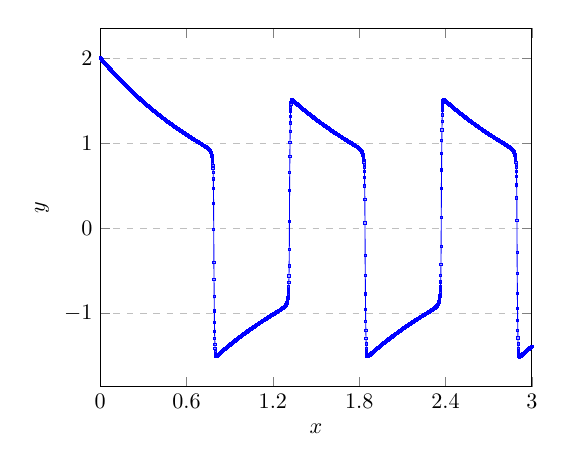
\begin{tikzpicture}[scale = 0.8]
    \begin{axis}[
        xlabel={$x$},
        ylabel={$y$},
        xmin=0, xmax=3,
        xtick={0,0.6,1.2,1.8,2.4,3},
        legend style={at={(1,-0.25)},
            anchor=north east},
        ymajorgrids=true,
        grid style=dashed,
    ]
    
    \addplot[
        color=blue,
        mark=square,
        mark size=0.5pt
    ]
    coordinates {
    (0,2)(0.001,1.99908)(0.002,1.99729)(0.003,1.99533)(0.004,1.99335)(0.005,1.99136)(0.006,1.98937)(0.007,1.98738)(0.008,1.98539)(0.009,1.98341)(0.01,1.98142)(0.011,1.97944)(0.012,1.97746)(0.013,1.97549)(0.014,1.97351)(0.015,1.97154)(0.016,1.96957)(0.017,1.9676)(0.018,1.96563)(0.019,1.96367)(0.02,1.9617)(0.021,1.95974)(0.022,1.95778)(0.023,1.95583)(0.024,1.95387)(0.025,1.95192)(0.026,1.94997)(0.027,1.94802)(0.028,1.94607)(0.029,1.94412)(0.03,1.94218)(0.031,1.94024)(0.032,1.9383)(0.033,1.93636)(0.034,1.93442)(0.035,1.93249)(0.036,1.93056)(0.037,1.92863)(0.038,1.9267)(0.039,1.92477)(0.04,1.92285)(0.041,1.92093)(0.042,1.91901)(0.043,1.91709)(0.044,1.91517)(0.045,1.91326)(0.046,1.91134)(0.047,1.90943)(0.048,1.90752)(0.049,1.90562)(0.05,1.90371)(0.051,1.90181)(0.052,1.89991)(0.053,1.89801)(0.054,1.89611)(0.055,1.89421)(0.056,1.89232)(0.057,1.89043)(0.058,1.88854)(0.059,1.88665)(0.06,1.88476)(0.061,1.88288)(0.062,1.881)(0.063,1.87911)(0.064,1.87724)(0.065,1.87536)(0.066,1.87348)(0.067,1.87161)(0.068,1.86974)(0.069,1.86787)(0.07,1.866)(0.071,1.86414)(0.072,1.86227)(0.073,1.86041)(0.074,1.85855)(0.075,1.85669)(0.076,1.85484)(0.077,1.85298)(0.078,1.85113)(0.079,1.84928)(0.08,1.84743)(0.081,1.84558)(0.082,1.84374)(0.083,1.84189)(0.084,1.84005)(0.085,1.83821)(0.086,1.83637)(0.087,1.83454)(0.088,1.8327)(0.089,1.83087)(0.09,1.82904)(0.091,1.82721)(0.092,1.82538)(0.093,1.82356)(0.094,1.82173)(0.095,1.81991)(0.096,1.81809)(0.097,1.81628)(0.098,1.81446)(0.099,1.81265)(0.1,1.81083)(0.101,1.80902)(0.102,1.80721)(0.103,1.80541)(0.104,1.8036)(0.105,1.8018)(0.106,1.8)(0.107,1.7982)(0.108,1.7964)(0.109,1.7946)(0.11,1.79281)(0.111,1.79101)(0.112,1.78922)(0.113,1.78743)(0.114,1.78565)(0.115,1.78386)(0.116,1.78208)(0.117,1.7803)(0.118,1.77851)(0.119,1.77674)(0.12,1.77496)(0.121,1.77318)(0.122,1.77141)(0.123,1.76964)(0.124,1.76787)(0.125,1.7661)(0.126,1.76434)(0.127,1.76257)(0.128,1.76081)(0.129,1.75905)(0.13,1.75729)(0.131,1.75553)(0.132,1.75378)(0.133,1.75202)(0.134,1.75027)(0.135,1.74852)(0.136,1.74677)(0.137,1.74503)(0.138,1.74328)(0.139,1.74154)(0.14,1.7398)(0.141,1.73806)(0.142,1.73632)(0.143,1.73458)(0.144,1.73285)(0.145,1.73111)(0.146,1.72938)(0.147,1.72765)(0.148,1.72593)(0.149,1.7242)(0.15,1.72248)(0.151,1.72075)(0.152,1.71903)(0.153,1.71731)(0.154,1.7156)(0.155,1.71388)(0.156,1.71217)(0.157,1.71045)(0.158,1.70874)(0.159,1.70703)(0.16,1.70533)(0.161,1.70362)(0.162,1.70192)(0.163,1.70022)(0.164,1.69851)(0.165,1.69682)(0.166,1.69512)(0.167,1.69342)(0.168,1.69173)(0.169,1.69004)(0.17,1.68835)(0.171,1.68666)(0.172,1.68497)(0.173,1.68329)(0.174,1.6816)(0.175,1.67992)(0.176,1.67824)(0.177,1.67656)(0.178,1.67489)(0.179,1.67321)(0.18,1.67154)(0.181,1.66987)(0.182,1.6682)(0.183,1.66653)(0.184,1.66486)(0.185,1.6632)(0.186,1.66153)(0.187,1.65987)(0.188,1.65821)(0.189,1.65655)(0.19,1.65489)(0.191,1.65324)(0.192,1.65159)(0.193,1.64993)(0.194,1.64828)(0.195,1.64663)(0.196,1.64499)(0.197,1.64334)(0.198,1.6417)(0.199,1.64006)(0.2,1.63842)(0.201,1.63678)(0.202,1.63514)(0.203,1.6335)(0.204,1.63187)(0.205,1.63024)(0.206,1.62861)(0.207,1.62698)(0.208,1.62535)(0.209,1.62373)(0.21,1.6221)(0.211,1.62048)(0.212,1.61886)(0.213,1.61724)(0.214,1.61562)(0.215,1.61401)(0.216,1.61239)(0.217,1.61078)(0.218,1.60917)(0.219,1.60756)(0.22,1.60595)(0.221,1.60434)(0.222,1.60274)(0.223,1.60113)(0.224,1.59953)(0.225,1.59793)(0.226,1.59633)(0.227,1.59474)(0.228,1.59314)(0.229,1.59155)(0.23,1.58996)(0.231,1.58837)(0.232,1.58678)(0.233,1.58519)(0.234,1.5836)(0.235,1.58202)(0.236,1.58044)(0.237,1.57886)(0.238,1.57728)(0.239,1.5757)(0.24,1.57412)(0.241,1.57255)(0.242,1.57097)(0.243,1.5694)(0.244,1.56783)(0.245,1.56626)(0.246,1.5647)(0.247,1.56313)(0.248,1.56157)(0.249,1.56001)(0.25,1.55845)(0.251,1.55689)(0.252,1.55533)(0.253,1.55377)(0.254,1.55222)(0.255,1.55066)(0.256,1.54911)(0.257,1.54756)(0.258,1.54602)(0.259,1.54447)(0.26,1.54292)(0.261,1.54138)(0.262,1.53984)(0.263,1.5383)(0.264,1.53676)(0.265,1.53522)(0.266,1.53368)(0.267,1.53215)(0.268,1.53062)(0.269,1.52909)(0.27,1.52756)(0.271,1.52603)(0.272,1.5245)(0.273,1.52297)(0.274,1.52145)(0.275,1.51993)(0.276,1.51841)(0.277,1.51689)(0.278,1.51537)(0.279,1.51385)(0.28,1.51234)(0.281,1.51083)(0.282,1.50931)(0.283,1.5078)(0.284,1.5063)(0.285,1.50479)(0.286,1.50328)(0.287,1.50178)(0.288,1.50028)(0.289,1.49877)(0.29,1.49728)(0.291,1.49578)(0.292,1.49428)(0.293,1.49278)(0.294,1.49129)(0.295,1.4898)(0.296,1.48831)(0.297,1.48682)(0.298,1.48533)(0.299,1.48384)(0.3,1.48236)(0.301,1.48088)(0.302,1.47939)(0.303,1.47791)(0.304,1.47643)(0.305,1.47496)(0.306,1.47348)(0.307,1.47201)(0.308,1.47053)(0.309,1.46906)(0.31,1.46759)(0.311,1.46612)(0.312,1.46466)(0.313,1.46319)(0.314,1.46173)(0.315,1.46026)(0.316,1.4588)(0.317,1.45734)(0.318,1.45588)(0.319,1.45443)(0.32,1.45297)(0.321,1.45152)(0.322,1.45006)(0.323,1.44861)(0.324,1.44716)(0.325,1.44571)(0.326,1.44427)(0.327,1.44282)(0.328,1.44138)(0.329,1.43993)(0.33,1.43849)(0.331,1.43705)(0.332,1.43561)(0.333,1.43418)(0.334,1.43274)(0.335,1.43131)(0.336,1.42988)(0.337,1.42844)(0.338,1.42701)(0.339,1.42559)(0.34,1.42416)(0.341,1.42273)(0.342,1.42131)(0.343,1.41989)(0.344,1.41846)(0.345,1.41705)(0.346,1.41563)(0.347,1.41421)(0.348,1.41279)(0.349,1.41138)(0.35,1.40997)(0.351,1.40856)(0.352,1.40715)(0.353,1.40574)(0.354,1.40433)(0.355,1.40292)(0.356,1.40152)(0.357,1.40012)(0.358,1.39871)(0.359,1.39731)(0.36,1.39591)(0.361,1.39452)(0.362,1.39312)(0.363,1.39173)(0.364,1.39033)(0.365,1.38894)(0.366,1.38755)(0.367,1.38616)(0.368,1.38477)(0.369,1.38339)(0.37,1.382)(0.371,1.38062)(0.372,1.37924)(0.373,1.37785)(0.374,1.37648)(0.375,1.3751)(0.376,1.37372)(0.377,1.37234)(0.378,1.37097)(0.379,1.3696)(0.38,1.36823)(0.381,1.36686)(0.382,1.36549)(0.383,1.36412)(0.384,1.36275)(0.385,1.36139)(0.386,1.36003)(0.387,1.35866)(0.388,1.3573)(0.389,1.35594)(0.39,1.35459)(0.391,1.35323)(0.392,1.35188)(0.393,1.35052)(0.394,1.34917)(0.395,1.34782)(0.396,1.34647)(0.397,1.34512)(0.398,1.34377)(0.399,1.34243)(0.4,1.34108)(0.401,1.33974)(0.402,1.3384)(0.403,1.33706)(0.404,1.33572)(0.405,1.33438)(0.406,1.33304)(0.407,1.33171)(0.408,1.33037)(0.409,1.32904)(0.41,1.32771)(0.411,1.32638)(0.412,1.32505)(0.413,1.32372)(0.414,1.3224)(0.415,1.32107)(0.416,1.31975)(0.417,1.31843)(0.418,1.31711)(0.419,1.31579)(0.42,1.31447)(0.421,1.31315)(0.422,1.31184)(0.423,1.31052)(0.424,1.30921)(0.425,1.3079)(0.426,1.30659)(0.427,1.30528)(0.428,1.30397)(0.429,1.30267)(0.43,1.30136)(0.431,1.30006)(0.432,1.29875)(0.433,1.29745)(0.434,1.29615)(0.435,1.29485)(0.436,1.29356)(0.437,1.29226)(0.438,1.29097)(0.439,1.28967)(0.44,1.28838)(0.441,1.28709)(0.442,1.2858)(0.443,1.28451)(0.444,1.28322)(0.445,1.28194)(0.446,1.28065)(0.447,1.27937)(0.448,1.27809)(0.449,1.27681)(0.45,1.27553)(0.451,1.27425)(0.452,1.27297)(0.453,1.2717)(0.454,1.27042)(0.455,1.26915)(0.456,1.26788)(0.457,1.2666)(0.458,1.26534)(0.459,1.26407)(0.46,1.2628)(0.461,1.26153)(0.462,1.26027)(0.463,1.25901)(0.464,1.25774)(0.465,1.25648)(0.466,1.25522)(0.467,1.25397)(0.468,1.25271)(0.469,1.25145)(0.47,1.2502)(0.471,1.24894)(0.472,1.24769)(0.473,1.24644)(0.474,1.24519)(0.475,1.24394)(0.476,1.2427)(0.477,1.24145)(0.478,1.2402)(0.479,1.23896)(0.48,1.23772)(0.481,1.23648)(0.482,1.23524)(0.483,1.234)(0.484,1.23276)(0.485,1.23153)(0.486,1.23029)(0.487,1.22906)(0.488,1.22782)(0.489,1.22659)(0.49,1.22536)(0.491,1.22413)(0.492,1.22291)(0.493,1.22168)(0.494,1.22045)(0.495,1.21923)(0.496,1.21801)(0.497,1.21678)(0.498,1.21556)(0.499,1.21434)(0.5,1.21313)(0.501,1.21191)(0.502,1.21069)(0.503,1.20948)(0.504,1.20826)(0.505,1.20705)(0.506,1.20584)(0.507,1.20463)(0.508,1.20342)(0.509,1.20222)(0.51,1.20101)(0.511,1.1998)(0.512,1.1986)(0.513,1.1974)(0.514,1.19619)(0.515,1.19499)(0.516,1.1938)(0.517,1.1926)(0.518,1.1914)(0.519,1.1902)(0.52,1.18901)(0.521,1.18782)(0.522,1.18662)(0.523,1.18543)(0.524,1.18424)(0.525,1.18305)(0.526,1.18187)(0.527,1.18068)(0.528,1.17949)(0.529,1.17831)(0.53,1.17713)(0.531,1.17594)(0.532,1.17476)(0.533,1.17358)(0.534,1.17241)(0.535,1.17123)(0.536,1.17005)(0.537,1.16888)(0.538,1.1677)(0.539,1.16653)(0.54,1.16536)(0.541,1.16419)(0.542,1.16302)(0.543,1.16185)(0.544,1.16068)(0.545,1.15952)(0.546,1.15835)(0.547,1.15719)(0.548,1.15602)(0.549,1.15486)(0.55,1.1537)(0.551,1.15254)(0.552,1.15138)(0.553,1.15023)(0.554,1.14907)(0.555,1.14792)(0.556,1.14676)(0.557,1.14561)(0.558,1.14446)(0.559,1.14331)(0.56,1.14216)(0.561,1.14101)(0.562,1.13986)(0.563,1.13872)(0.564,1.13757)(0.565,1.13643)(0.566,1.13528)(0.567,1.13414)(0.568,1.133)(0.569,1.13186)(0.57,1.13072)(0.571,1.12959)(0.572,1.12845)(0.573,1.12731)(0.574,1.12618)(0.575,1.12505)(0.576,1.12392)(0.577,1.12278)(0.578,1.12165)(0.579,1.12053)(0.58,1.1194)(0.581,1.11827)(0.582,1.11715)(0.583,1.11602)(0.584,1.1149)(0.585,1.11377)(0.586,1.11265)(0.587,1.11153)(0.588,1.11041)(0.589,1.10929)(0.59,1.10818)(0.591,1.10706)(0.592,1.10595)(0.593,1.10483)(0.594,1.10372)(0.595,1.10261)(0.596,1.1015)(0.597,1.10038)(0.598,1.09928)(0.599,1.09817)(0.6,1.09706)(0.601,1.09595)(0.602,1.09485)(0.603,1.09375)(0.604,1.09264)(0.605,1.09154)(0.606,1.09044)(0.607,1.08934)(0.608,1.08824)(0.609,1.08714)(0.61,1.08605)(0.611,1.08495)(0.612,1.08385)(0.613,1.08276)(0.614,1.08167)(0.615,1.08057)(0.616,1.07948)(0.617,1.07839)(0.618,1.0773)(0.619,1.07622)(0.62,1.07513)(0.621,1.07404)(0.622,1.07296)(0.623,1.07187)(0.624,1.07079)(0.625,1.0697)(0.626,1.06862)(0.627,1.06754)(0.628,1.06646)(0.629,1.06538)(0.63,1.06431)(0.631,1.06323)(0.632,1.06215)(0.633,1.06108)(0.634,1.06)(0.635,1.05893)(0.636,1.05786)(0.637,1.05678)(0.638,1.05571)(0.639,1.05464)(0.64,1.05357)(0.641,1.05251)(0.642,1.05144)(0.643,1.05037)(0.644,1.04931)(0.645,1.04824)(0.646,1.04718)(0.647,1.04611)(0.648,1.04505)(0.649,1.04399)(0.65,1.04293)(0.651,1.04187)(0.652,1.04081)(0.653,1.03975)(0.654,1.03869)(0.655,1.03763)(0.656,1.03658)(0.657,1.03552)(0.658,1.03447)(0.659,1.03341)(0.66,1.03236)(0.661,1.03131)(0.662,1.03025)(0.663,1.0292)(0.664,1.02815)(0.665,1.0271)(0.666,1.02605)(0.667,1.025)(0.668,1.02395)(0.669,1.02291)(0.67,1.02186)(0.671,1.02081)(0.672,1.01977)(0.673,1.01872)(0.674,1.01767)(0.675,1.01663)(0.676,1.01559)(0.677,1.01454)(0.678,1.0135)(0.679,1.01245)(0.68,1.01141)(0.681,1.01037)(0.682,1.00933)(0.683,1.00829)(0.684,1.00724)(0.685,1.0062)(0.686,1.00516)(0.687,1.00412)(0.688,1.00308)(0.689,1.00204)(0.69,1.001)(0.691,0.999958)(0.692,0.998917)(0.693,0.997876)(0.694,0.996835)(0.695,0.995794)(0.696,0.994752)(0.697,0.99371)(0.698,0.992668)(0.699,0.991626)(0.7,0.990583)(0.701,0.989539)(0.702,0.988495)(0.703,0.98745)(0.704,0.986404)(0.705,0.985358)(0.706,0.98431)(0.707,0.983261)(0.708,0.982211)(0.709,0.98116)(0.71,0.980108)(0.711,0.979053)(0.712,0.977998)(0.713,0.97694)(0.714,0.97588)(0.715,0.974818)(0.716,0.973754)(0.717,0.972688)(0.718,0.971618)(0.719,0.970546)(0.72,0.96947)(0.721,0.968391)(0.722,0.967309)(0.723,0.966222)(0.724,0.965131)(0.725,0.964036)(0.726,0.962935)(0.727,0.961829)(0.728,0.960718)(0.729,0.9596)(0.73,0.958475)(0.731,0.957343)(0.732,0.956203)(0.733,0.955055)(0.734,0.953898)(0.735,0.95273)(0.736,0.951552)(0.737,0.950363)(0.738,0.949161)(0.739,0.947946)(0.74,0.946716)(0.741,0.94547)(0.742,0.944207)(0.743,0.942925)(0.744,0.941623)(0.745,0.940298)(0.746,0.93895)(0.747,0.937575)(0.748,0.936172)(0.749,0.934737)(0.75,0.933267)(0.751,0.93176)(0.752,0.930212)(0.753,0.928618)(0.754,0.926973)(0.755,0.925274)(0.756,0.923513)(0.757,0.921684)(0.758,0.91978)(0.759,0.917792)(0.76,0.915711)(0.761,0.913525)(0.762,0.911222)(0.763,0.908787)(0.764,0.906203)(0.765,0.90345)(0.766,0.900506)(0.767,0.897344)(0.768,0.89393)(0.769,0.890227)(0.77,0.88619)(0.771,0.881762)(0.772,0.876877)(0.773,0.87145)(0.774,0.865378)(0.775,0.85853)(0.776,0.850738)(0.777,0.841783)(0.778,0.831379)(0.779,0.819134)(0.78,0.804511)(0.781,0.786741)(0.782,0.764697)(0.783,0.736653)(0.784,0.699845)(0.785,0.649579)(0.786,0.577367)(0.787,0.466764)(0.788,0.284912)(0.789,-0.0206831)(0.79,-0.401342)(0.791,-0.606841)(0.792,-0.809452)(0.793,-0.976669)(0.794,-1.11124)(0.795,-1.21855)(0.796,-1.3029)(0.797,-1.3676)(0.798,-1.4156)(0.799,-1.4498)(0.8,-1.47317)(0.801,-1.48848)(0.802,-1.49809)(0.803,-1.50382)(0.804,-1.50696)(0.805,-1.50842)(0.806,-1.50881)(0.807,-1.5085)(0.808,-1.50776)(0.809,-1.50673)(0.81,-1.50553)(0.811,-1.50422)(0.812,-1.50284)(0.813,-1.50142)(0.814,-1.49997)(0.815,-1.4985)(0.816,-1.49702)(0.817,-1.49553)(0.818,-1.49405)(0.819,-1.49256)(0.82,-1.49107)(0.821,-1.48958)(0.822,-1.48809)(0.823,-1.4866)(0.824,-1.48511)(0.825,-1.48363)(0.826,-1.48214)(0.827,-1.48066)(0.828,-1.47918)(0.829,-1.4777)(0.83,-1.47622)(0.831,-1.47474)(0.832,-1.47326)(0.833,-1.47179)(0.834,-1.47032)(0.835,-1.46885)(0.836,-1.46738)(0.837,-1.46591)(0.838,-1.46444)(0.839,-1.46297)(0.84,-1.46151)(0.841,-1.46005)(0.842,-1.45859)(0.843,-1.45713)(0.844,-1.45567)(0.845,-1.45421)(0.846,-1.45276)(0.847,-1.4513)(0.848,-1.44985)(0.849,-1.4484)(0.85,-1.44695)(0.851,-1.4455)(0.852,-1.44405)(0.853,-1.44261)(0.854,-1.44116)(0.855,-1.43972)(0.856,-1.43828)(0.857,-1.43684)(0.858,-1.4354)(0.859,-1.43397)(0.86,-1.43253)(0.861,-1.4311)(0.862,-1.42966)(0.863,-1.42823)(0.864,-1.4268)(0.865,-1.42538)(0.866,-1.42395)(0.867,-1.42252)(0.868,-1.4211)(0.869,-1.41968)(0.87,-1.41826)(0.871,-1.41684)(0.872,-1.41542)(0.873,-1.414)(0.874,-1.41259)(0.875,-1.41117)(0.876,-1.40976)(0.877,-1.40835)(0.878,-1.40694)(0.879,-1.40553)(0.88,-1.40412)(0.881,-1.40272)(0.882,-1.40131)(0.883,-1.39991)(0.884,-1.39851)(0.885,-1.39711)(0.886,-1.39571)(0.887,-1.39431)(0.888,-1.39292)(0.889,-1.39152)(0.89,-1.39013)(0.891,-1.38874)(0.892,-1.38735)(0.893,-1.38596)(0.894,-1.38457)(0.895,-1.38318)(0.896,-1.3818)(0.897,-1.38042)(0.898,-1.37903)(0.899,-1.37765)(0.9,-1.37627)(0.901,-1.37489)(0.902,-1.37352)(0.903,-1.37214)(0.904,-1.37077)(0.905,-1.3694)(0.906,-1.36803)(0.907,-1.36666)(0.908,-1.36529)(0.909,-1.36392)(0.91,-1.36255)(0.911,-1.36119)(0.912,-1.35983)(0.913,-1.35846)(0.914,-1.3571)(0.915,-1.35575)(0.916,-1.35439)(0.917,-1.35303)(0.918,-1.35168)(0.919,-1.35032)(0.92,-1.34897)(0.921,-1.34762)(0.922,-1.34627)(0.923,-1.34492)(0.924,-1.34357)(0.925,-1.34223)(0.926,-1.34088)(0.927,-1.33954)(0.928,-1.3382)(0.929,-1.33686)(0.93,-1.33552)(0.931,-1.33418)(0.932,-1.33285)(0.933,-1.33151)(0.934,-1.33018)(0.935,-1.32885)(0.936,-1.32751)(0.937,-1.32618)(0.938,-1.32486)(0.939,-1.32353)(0.94,-1.3222)(0.941,-1.32088)(0.942,-1.31956)(0.943,-1.31823)(0.944,-1.31691)(0.945,-1.31559)(0.946,-1.31428)(0.947,-1.31296)(0.948,-1.31164)(0.949,-1.31033)(0.95,-1.30902)(0.951,-1.30771)(0.952,-1.3064)(0.953,-1.30509)(0.954,-1.30378)(0.955,-1.30247)(0.956,-1.30117)(0.957,-1.29987)(0.958,-1.29856)(0.959,-1.29726)(0.96,-1.29596)(0.961,-1.29466)(0.962,-1.29337)(0.963,-1.29207)(0.964,-1.29078)(0.965,-1.28948)(0.966,-1.28819)(0.967,-1.2869)(0.968,-1.28561)(0.969,-1.28432)(0.97,-1.28303)(0.971,-1.28175)(0.972,-1.28046)(0.973,-1.27918)(0.974,-1.2779)(0.975,-1.27662)(0.976,-1.27534)(0.977,-1.27406)(0.978,-1.27278)(0.979,-1.27151)(0.98,-1.27023)(0.981,-1.26896)(0.982,-1.26769)(0.983,-1.26642)(0.984,-1.26515)(0.985,-1.26388)(0.986,-1.26261)(0.987,-1.26135)(0.988,-1.26008)(0.989,-1.25882)(0.99,-1.25756)(0.991,-1.2563)(0.992,-1.25504)(0.993,-1.25378)(0.994,-1.25252)(0.995,-1.25127)(0.996,-1.25001)(0.997,-1.24876)(0.998,-1.24751)(0.999,-1.24626)(1,-1.24501)(1.001,-1.24376)(1.002,-1.24251)(1.003,-1.24127)(1.004,-1.24002)(1.005,-1.23878)(1.006,-1.23754)(1.007,-1.2363)(1.008,-1.23506)(1.009,-1.23382)(1.01,-1.23258)(1.011,-1.23134)(1.012,-1.23011)(1.013,-1.22888)(1.014,-1.22764)(1.015,-1.22641)(1.016,-1.22518)(1.017,-1.22395)(1.018,-1.22272)(1.019,-1.2215)(1.02,-1.22027)(1.021,-1.21905)(1.022,-1.21783)(1.023,-1.2166)(1.024,-1.21538)(1.025,-1.21416)(1.026,-1.21295)(1.027,-1.21173)(1.028,-1.21051)(1.029,-1.2093)(1.03,-1.20809)(1.031,-1.20687)(1.032,-1.20566)(1.033,-1.20445)(1.034,-1.20325)(1.035,-1.20204)(1.036,-1.20083)(1.037,-1.19963)(1.038,-1.19842)(1.039,-1.19722)(1.04,-1.19602)(1.041,-1.19482)(1.042,-1.19362)(1.043,-1.19242)(1.044,-1.19122)(1.045,-1.19003)(1.046,-1.18883)(1.047,-1.18764)(1.048,-1.18645)(1.049,-1.18526)(1.05,-1.18407)(1.051,-1.18288)(1.052,-1.18169)(1.053,-1.1805)(1.054,-1.17932)(1.055,-1.17814)(1.056,-1.17695)(1.057,-1.17577)(1.058,-1.17459)(1.059,-1.17341)(1.06,-1.17223)(1.061,-1.17105)(1.062,-1.16988)(1.063,-1.1687)(1.064,-1.16753)(1.065,-1.16636)(1.066,-1.16519)(1.067,-1.16402)(1.068,-1.16285)(1.069,-1.16168)(1.07,-1.16051)(1.071,-1.15934)(1.072,-1.15818)(1.073,-1.15702)(1.074,-1.15585)(1.075,-1.15469)(1.076,-1.15353)(1.077,-1.15237)(1.078,-1.15121)(1.079,-1.15006)(1.08,-1.1489)(1.081,-1.14775)(1.082,-1.14659)(1.083,-1.14544)(1.084,-1.14429)(1.085,-1.14314)(1.086,-1.14199)(1.087,-1.14084)(1.088,-1.13969)(1.089,-1.13855)(1.09,-1.1374)(1.091,-1.13626)(1.092,-1.13512)(1.093,-1.13398)(1.094,-1.13283)(1.095,-1.1317)(1.096,-1.13056)(1.097,-1.12942)(1.098,-1.12828)(1.099,-1.12715)(1.1,-1.12601)(1.101,-1.12488)(1.102,-1.12375)(1.103,-1.12262)(1.104,-1.12149)(1.105,-1.12036)(1.106,-1.11923)(1.107,-1.11811)(1.108,-1.11698)(1.109,-1.11586)(1.11,-1.11473)(1.111,-1.11361)(1.112,-1.11249)(1.113,-1.11137)(1.114,-1.11025)(1.115,-1.10913)(1.116,-1.10801)(1.117,-1.1069)(1.118,-1.10578)(1.119,-1.10467)(1.12,-1.10355)(1.121,-1.10244)(1.122,-1.10133)(1.123,-1.10022)(1.124,-1.09911)(1.125,-1.098)(1.126,-1.0969)(1.127,-1.09579)(1.128,-1.09469)(1.129,-1.09358)(1.13,-1.09248)(1.131,-1.09138)(1.132,-1.09028)(1.133,-1.08918)(1.134,-1.08808)(1.135,-1.08698)(1.136,-1.08588)(1.137,-1.08479)(1.138,-1.08369)(1.139,-1.0826)(1.14,-1.08151)(1.141,-1.08041)(1.142,-1.07932)(1.143,-1.07823)(1.144,-1.07714)(1.145,-1.07606)(1.146,-1.07497)(1.147,-1.07388)(1.148,-1.0728)(1.149,-1.07171)(1.15,-1.07063)(1.151,-1.06955)(1.152,-1.06846)(1.153,-1.06738)(1.154,-1.0663)(1.155,-1.06523)(1.156,-1.06415)(1.157,-1.06307)(1.158,-1.06199)(1.159,-1.06092)(1.16,-1.05984)(1.161,-1.05877)(1.162,-1.0577)(1.163,-1.05663)(1.164,-1.05556)(1.165,-1.05449)(1.166,-1.05342)(1.167,-1.05235)(1.168,-1.05128)(1.169,-1.05021)(1.17,-1.04915)(1.171,-1.04808)(1.172,-1.04702)(1.173,-1.04596)(1.174,-1.04489)(1.175,-1.04383)(1.176,-1.04277)(1.177,-1.04171)(1.178,-1.04065)(1.179,-1.03959)(1.18,-1.03854)(1.181,-1.03748)(1.182,-1.03642)(1.183,-1.03537)(1.184,-1.03431)(1.185,-1.03326)(1.186,-1.0322)(1.187,-1.03115)(1.188,-1.0301)(1.189,-1.02905)(1.19,-1.028)(1.191,-1.02695)(1.192,-1.0259)(1.193,-1.02485)(1.194,-1.0238)(1.195,-1.02275)(1.196,-1.0217)(1.197,-1.02066)(1.198,-1.01961)(1.199,-1.01857)(1.2,-1.01752)(1.201,-1.01648)(1.202,-1.01543)(1.203,-1.01439)(1.204,-1.01334)(1.205,-1.0123)(1.206,-1.01126)(1.207,-1.01022)(1.208,-1.00917)(1.209,-1.00813)(1.21,-1.00709)(1.211,-1.00605)(1.212,-1.00501)(1.213,-1.00397)(1.214,-1.00293)(1.215,-1.00189)(1.216,-1.00085)(1.217,-0.999805)(1.218,-0.998764)(1.219,-0.997723)(1.22,-0.996682)(1.221,-0.995641)(1.222,-0.994599)(1.223,-0.993557)(1.224,-0.992515)(1.225,-0.991472)(1.226,-0.990429)(1.227,-0.989386)(1.228,-0.988341)(1.229,-0.987296)(1.23,-0.98625)(1.231,-0.985204)(1.232,-0.984156)(1.233,-0.983107)(1.234,-0.982057)(1.235,-0.981006)(1.236,-0.979953)(1.237,-0.978898)(1.238,-0.977842)(1.239,-0.976784)(1.24,-0.975724)(1.241,-0.974662)(1.242,-0.973598)(1.243,-0.972531)(1.244,-0.971461)(1.245,-0.970388)(1.246,-0.969312)(1.247,-0.968233)(1.248,-0.967149)(1.249,-0.966062)(1.25,-0.964971)(1.251,-0.963874)(1.252,-0.962773)(1.253,-0.961666)(1.254,-0.960554)(1.255,-0.959435)(1.256,-0.958309)(1.257,-0.957176)(1.258,-0.956035)(1.259,-0.954886)(1.26,-0.953727)(1.261,-0.952558)(1.262,-0.951378)(1.263,-0.950187)(1.264,-0.948983)(1.265,-0.947766)(1.266,-0.946534)(1.267,-0.945285)(1.268,-0.94402)(1.269,-0.942735)(1.27,-0.94143)(1.271,-0.940102)(1.272,-0.93875)(1.273,-0.937371)(1.274,-0.935963)(1.275,-0.934523)(1.276,-0.933048)(1.277,-0.931535)(1.278,-0.929981)(1.279,-0.928379)(1.28,-0.926727)(1.281,-0.925019)(1.282,-0.923249)(1.283,-0.921409)(1.284,-0.919494)(1.285,-0.917493)(1.286,-0.915397)(1.287,-0.913194)(1.288,-0.910873)(1.289,-0.908417)(1.29,-0.90581)(1.291,-0.90303)(1.292,-0.900056)(1.293,-0.896859)(1.294,-0.893405)(1.295,-0.889656)(1.296,-0.885565)(1.297,-0.881075)(1.298,-0.876116)(1.299,-0.870601)(1.3,-0.864424)(1.301,-0.857449)(1.302,-0.849501)(1.303,-0.840354)(1.304,-0.829706)(1.305,-0.81715)(1.306,-0.802119)(1.307,-0.783803)(1.308,-0.761004)(1.309,-0.73188)(1.31,-0.693451)(1.311,-0.640622)(1.312,-0.564074)(1.313,-0.445604)(1.314,-0.249041)(1.315,0.0773521)(1.316,0.441947)(1.317,0.650183)(1.318,0.845412)(1.319,1.00539)(1.32,1.134)(1.321,1.23637)(1.322,1.31651)(1.323,1.37764)(1.324,1.42265)(1.325,1.45446)(1.326,1.47603)(1.327,1.49006)(1.328,1.49878)(1.329,1.50392)(1.33,1.50668)(1.331,1.5079)(1.332,1.50812)(1.333,1.50772)(1.334,1.50691)(1.335,1.50585)(1.336,1.50462)(1.337,1.5033)(1.338,1.50191)(1.339,1.50048)(1.34,1.49902)(1.341,1.49755)(1.342,1.49607)(1.343,1.49459)(1.344,1.4931)(1.345,1.49161)(1.346,1.49012)(1.347,1.48863)(1.348,1.48715)(1.349,1.48566)(1.35,1.48417)(1.351,1.48269)(1.352,1.4812)(1.353,1.47972)(1.354,1.47824)(1.355,1.47676)(1.356,1.47528)(1.357,1.47381)(1.358,1.47233)(1.359,1.47086)(1.36,1.46939)(1.361,1.46792)(1.362,1.46645)(1.363,1.46498)(1.364,1.46351)(1.365,1.46205)(1.366,1.46059)(1.367,1.45912)(1.368,1.45766)(1.369,1.45621)(1.37,1.45475)(1.371,1.45329)(1.372,1.45184)(1.373,1.45038)(1.374,1.44893)(1.375,1.44748)(1.376,1.44603)(1.377,1.44459)(1.378,1.44314)(1.379,1.4417)(1.38,1.44025)(1.381,1.43881)(1.382,1.43737)(1.383,1.43593)(1.384,1.4345)(1.385,1.43306)(1.386,1.43163)(1.387,1.43019)(1.388,1.42876)(1.389,1.42733)(1.39,1.4259)(1.391,1.42447)(1.392,1.42305)(1.393,1.42162)(1.394,1.4202)(1.395,1.41878)(1.396,1.41736)(1.397,1.41594)(1.398,1.41452)(1.399,1.41311)(1.4,1.41169)(1.401,1.41028)(1.402,1.40887)(1.403,1.40746)(1.404,1.40605)(1.405,1.40464)(1.406,1.40323)(1.407,1.40183)(1.408,1.40043)(1.409,1.39902)(1.41,1.39762)(1.411,1.39622)(1.412,1.39483)(1.413,1.39343)(1.414,1.39204)(1.415,1.39064)(1.416,1.38925)(1.417,1.38786)(1.418,1.38647)(1.419,1.38508)(1.42,1.38369)(1.421,1.38231)(1.422,1.38092)(1.423,1.37954)(1.424,1.37816)(1.425,1.37678)(1.426,1.3754)(1.427,1.37403)(1.428,1.37265)(1.429,1.37127)(1.43,1.3699)(1.431,1.36853)(1.432,1.36716)(1.433,1.36579)(1.434,1.36442)(1.435,1.36306)(1.436,1.36169)(1.437,1.36033)(1.438,1.35897)(1.439,1.35761)(1.44,1.35625)(1.441,1.35489)(1.442,1.35353)(1.443,1.35218)(1.444,1.35082)(1.445,1.34947)(1.446,1.34812)(1.447,1.34677)(1.448,1.34542)(1.449,1.34407)(1.45,1.34272)(1.451,1.34138)(1.452,1.34004)(1.453,1.33869)(1.454,1.33735)(1.455,1.33601)(1.456,1.33468)(1.457,1.33334)(1.458,1.332)(1.459,1.33067)(1.46,1.32934)(1.461,1.32801)(1.462,1.32667)(1.463,1.32535)(1.464,1.32402)(1.465,1.32269)(1.466,1.32137)(1.467,1.32004)(1.468,1.31872)(1.469,1.3174)(1.47,1.31608)(1.471,1.31476)(1.472,1.31345)(1.473,1.31213)(1.474,1.31081)(1.475,1.3095)(1.476,1.30819)(1.477,1.30688)(1.478,1.30557)(1.479,1.30426)(1.48,1.30296)(1.481,1.30165)(1.482,1.30035)(1.483,1.29904)(1.484,1.29774)(1.485,1.29644)(1.486,1.29514)(1.487,1.29384)(1.488,1.29255)(1.489,1.29125)(1.49,1.28996)(1.491,1.28867)(1.492,1.28737)(1.493,1.28608)(1.494,1.2848)(1.495,1.28351)(1.496,1.28222)(1.497,1.28094)(1.498,1.27965)(1.499,1.27837)(1.5,1.27709)(1.501,1.27581)(1.502,1.27453)(1.503,1.27325)(1.504,1.27198)(1.505,1.2707)(1.506,1.26943)(1.507,1.26816)(1.508,1.26689)(1.509,1.26562)(1.51,1.26435)(1.511,1.26308)(1.512,1.26181)(1.513,1.26055)(1.514,1.25929)(1.515,1.25802)(1.516,1.25676)(1.517,1.2555)(1.518,1.25424)(1.519,1.25299)(1.52,1.25173)(1.521,1.25048)(1.522,1.24922)(1.523,1.24797)(1.524,1.24672)(1.525,1.24547)(1.526,1.24422)(1.527,1.24297)(1.528,1.24173)(1.529,1.24048)(1.53,1.23924)(1.531,1.23799)(1.532,1.23675)(1.533,1.23551)(1.534,1.23427)(1.535,1.23304)(1.536,1.2318)(1.537,1.23056)(1.538,1.22933)(1.539,1.2281)(1.54,1.22686)(1.541,1.22563)(1.542,1.22441)(1.543,1.22318)(1.544,1.22195)(1.545,1.22072)(1.546,1.2195)(1.547,1.21828)(1.548,1.21705)(1.549,1.21583)(1.55,1.21461)(1.551,1.2134)(1.552,1.21218)(1.553,1.21096)(1.554,1.20975)(1.555,1.20853)(1.556,1.20732)(1.557,1.20611)(1.558,1.2049)(1.559,1.20369)(1.56,1.20248)(1.561,1.20128)(1.562,1.20007)(1.563,1.19887)(1.564,1.19766)(1.565,1.19646)(1.566,1.19526)(1.567,1.19406)(1.568,1.19286)(1.569,1.19167)(1.57,1.19047)(1.571,1.18927)(1.572,1.18808)(1.573,1.18689)(1.574,1.1857)(1.575,1.18451)(1.576,1.18332)(1.577,1.18213)(1.578,1.18094)(1.579,1.17976)(1.58,1.17857)(1.581,1.17739)(1.582,1.17621)(1.583,1.17502)(1.584,1.17384)(1.585,1.17267)(1.586,1.17149)(1.587,1.17031)(1.588,1.16914)(1.589,1.16796)(1.59,1.16679)(1.591,1.16562)(1.592,1.16445)(1.593,1.16328)(1.594,1.16211)(1.595,1.16094)(1.596,1.15977)(1.597,1.15861)(1.598,1.15744)(1.599,1.15628)(1.6,1.15512)(1.601,1.15396)(1.602,1.1528)(1.603,1.15164)(1.604,1.15048)(1.605,1.14933)(1.606,1.14817)(1.607,1.14702)(1.608,1.14587)(1.609,1.14471)(1.61,1.14356)(1.611,1.14241)(1.612,1.14126)(1.613,1.14012)(1.614,1.13897)(1.615,1.13783)(1.616,1.13668)(1.617,1.13554)(1.618,1.1344)(1.619,1.13325)(1.62,1.13212)(1.621,1.13098)(1.622,1.12984)(1.623,1.1287)(1.624,1.12757)(1.625,1.12643)(1.626,1.1253)(1.627,1.12417)(1.628,1.12303)(1.629,1.1219)(1.63,1.12078)(1.631,1.11965)(1.632,1.11852)(1.633,1.11739)(1.634,1.11627)(1.635,1.11515)(1.636,1.11402)(1.637,1.1129)(1.638,1.11178)(1.639,1.11066)(1.64,1.10954)(1.641,1.10842)(1.642,1.10731)(1.643,1.10619)(1.644,1.10508)(1.645,1.10396)(1.646,1.10285)(1.647,1.10174)(1.648,1.10063)(1.649,1.09952)(1.65,1.09841)(1.651,1.09731)(1.652,1.0962)(1.653,1.09509)(1.654,1.09399)(1.655,1.09289)(1.656,1.09178)(1.657,1.09068)(1.658,1.08958)(1.659,1.08848)(1.66,1.08739)(1.661,1.08629)(1.662,1.08519)(1.663,1.0841)(1.664,1.083)(1.665,1.08191)(1.666,1.08082)(1.667,1.07972)(1.668,1.07863)(1.669,1.07754)(1.67,1.07646)(1.671,1.07537)(1.672,1.07428)(1.673,1.0732)(1.674,1.07211)(1.675,1.07103)(1.676,1.06994)(1.677,1.06886)(1.678,1.06778)(1.679,1.0667)(1.68,1.06562)(1.681,1.06454)(1.682,1.06347)(1.683,1.06239)(1.684,1.06131)(1.685,1.06024)(1.686,1.05917)(1.687,1.05809)(1.688,1.05702)(1.689,1.05595)(1.69,1.05488)(1.691,1.05381)(1.692,1.05274)(1.693,1.05167)(1.694,1.05061)(1.695,1.04954)(1.696,1.04848)(1.697,1.04741)(1.698,1.04635)(1.699,1.04529)(1.7,1.04422)(1.701,1.04316)(1.702,1.0421)(1.703,1.04104)(1.704,1.03998)(1.705,1.03893)(1.706,1.03787)(1.707,1.03681)(1.708,1.03576)(1.709,1.0347)(1.71,1.03365)(1.711,1.03259)(1.712,1.03154)(1.713,1.03049)(1.714,1.02943)(1.715,1.02838)(1.716,1.02733)(1.717,1.02628)(1.718,1.02523)(1.719,1.02419)(1.72,1.02314)(1.721,1.02209)(1.722,1.02104)(1.723,1.02)(1.724,1.01895)(1.725,1.01791)(1.726,1.01686)(1.727,1.01582)(1.728,1.01477)(1.729,1.01373)(1.73,1.01269)(1.731,1.01164)(1.732,1.0106)(1.733,1.00956)(1.734,1.00852)(1.735,1.00748)(1.736,1.00643)(1.737,1.00539)(1.738,1.00435)(1.739,1.00331)(1.74,1.00227)(1.741,1.00123)(1.742,1.00019)(1.743,0.999147)(1.744,0.998107)(1.745,0.997066)(1.746,0.996024)(1.747,0.994983)(1.748,0.993941)(1.749,0.992899)(1.75,0.991857)(1.751,0.990814)(1.752,0.98977)(1.753,0.988726)(1.754,0.987682)(1.755,0.986636)(1.756,0.98559)(1.757,0.984542)(1.758,0.983494)(1.759,0.982444)(1.76,0.981393)(1.761,0.980341)(1.762,0.979287)(1.763,0.978232)(1.764,0.977174)(1.765,0.976115)(1.766,0.975054)(1.767,0.97399)(1.768,0.972924)(1.769,0.971855)(1.77,0.970784)(1.771,0.969709)(1.772,0.968631)(1.773,0.967549)(1.774,0.966463)(1.775,0.965373)(1.776,0.964279)(1.777,0.96318)(1.778,0.962075)(1.779,0.960964)(1.78,0.959848)(1.781,0.958725)(1.782,0.957595)(1.783,0.956457)(1.784,0.95531)(1.785,0.954155)(1.786,0.95299)(1.787,0.951814)(1.788,0.950628)(1.789,0.949429)(1.79,0.948216)(1.791,0.94699)(1.792,0.945747)(1.793,0.944488)(1.794,0.943211)(1.795,0.941913)(1.796,0.940594)(1.797,0.939251)(1.798,0.937882)(1.799,0.936485)(1.8,0.935058)(1.801,0.933596)(1.802,0.932098)(1.803,0.930559)(1.804,0.928975)(1.805,0.927342)(1.806,0.925656)(1.807,0.923909)(1.808,0.922096)(1.809,0.920209)(1.81,0.918241)(1.811,0.916181)(1.812,0.914019)(1.813,0.911743)(1.814,0.909339)(1.815,0.906789)(1.816,0.904076)(1.817,0.901177)(1.818,0.898065)(1.819,0.89471)(1.82,0.891075)(1.821,0.887116)(1.822,0.882781)(1.823,0.878003)(1.824,0.872704)(1.825,0.866786)(1.826,0.860122)(1.827,0.852556)(1.828,0.843881)(1.829,0.833828)(1.83,0.822031)(1.831,0.807991)(1.832,0.791)(1.833,0.770027)(1.834,0.743505)(1.835,0.708956)(1.836,0.662229)(1.837,0.595923)(1.838,0.495909)(1.839,0.333916)(1.84,0.0597105)(1.841,-0.327051)(1.842,-0.555619)(1.843,-0.776561)(1.844,-0.953588)(1.845,-1.09491)(1.846,-1.20739)(1.847,-1.29591)(1.848,-1.36406)(1.849,-1.41486)(1.85,-1.45123)(1.851,-1.47618)(1.852,-1.49258)(1.853,-1.5029)(1.854,-1.50907)(1.855,-1.51248)(1.856,-1.5141)(1.857,-1.51458)(1.858,-1.51432)(1.859,-1.51361)(1.86,-1.51259)(1.861,-1.5114)(1.862,-1.51009)(1.863,-1.5087)(1.864,-1.50728)(1.865,-1.50582)(1.866,-1.50434)(1.867,-1.50286)(1.868,-1.50137)(1.869,-1.49988)(1.87,-1.49838)(1.871,-1.49688)(1.872,-1.49539)(1.873,-1.49389)(1.874,-1.4924)(1.875,-1.49091)(1.876,-1.48942)(1.877,-1.48793)(1.878,-1.48644)(1.879,-1.48495)(1.88,-1.48346)(1.881,-1.48198)(1.882,-1.4805)(1.883,-1.47901)(1.884,-1.47753)(1.885,-1.47606)(1.886,-1.47458)(1.887,-1.4731)(1.888,-1.47163)(1.889,-1.47016)(1.89,-1.46868)(1.891,-1.46721)(1.892,-1.46575)(1.893,-1.46428)(1.894,-1.46281)(1.895,-1.46135)(1.896,-1.45989)(1.897,-1.45843)(1.898,-1.45697)(1.899,-1.45551)(1.9,-1.45405)(1.901,-1.4526)(1.902,-1.45114)(1.903,-1.44969)(1.904,-1.44824)(1.905,-1.44679)(1.906,-1.44534)(1.907,-1.4439)(1.908,-1.44245)(1.909,-1.44101)(1.91,-1.43956)(1.911,-1.43812)(1.912,-1.43668)(1.913,-1.43525)(1.914,-1.43381)(1.915,-1.43237)(1.916,-1.43094)(1.917,-1.42951)(1.918,-1.42808)(1.919,-1.42665)(1.92,-1.42522)(1.921,-1.42379)(1.922,-1.42237)(1.923,-1.42094)(1.924,-1.41952)(1.925,-1.4181)(1.926,-1.41668)(1.927,-1.41526)(1.928,-1.41385)(1.929,-1.41243)(1.93,-1.41102)(1.931,-1.4096)(1.932,-1.40819)(1.933,-1.40678)(1.934,-1.40538)(1.935,-1.40397)(1.936,-1.40256)(1.937,-1.40116)(1.938,-1.39976)(1.939,-1.39835)(1.94,-1.39695)(1.941,-1.39556)(1.942,-1.39416)(1.943,-1.39276)(1.944,-1.39137)(1.945,-1.38998)(1.946,-1.38858)(1.947,-1.38719)(1.948,-1.38581)(1.949,-1.38442)(1.95,-1.38303)(1.951,-1.38165)(1.952,-1.38026)(1.953,-1.37888)(1.954,-1.3775)(1.955,-1.37612)(1.956,-1.37474)(1.957,-1.37337)(1.958,-1.37199)(1.959,-1.37062)(1.96,-1.36925)(1.961,-1.36787)(1.962,-1.3665)(1.963,-1.36514)(1.964,-1.36377)(1.965,-1.3624)(1.966,-1.36104)(1.967,-1.35968)(1.968,-1.35832)(1.969,-1.35696)(1.97,-1.3556)(1.971,-1.35424)(1.972,-1.35288)(1.973,-1.35153)(1.974,-1.35017)(1.975,-1.34882)(1.976,-1.34747)(1.977,-1.34612)(1.978,-1.34477)(1.979,-1.34343)(1.98,-1.34208)(1.981,-1.34074)(1.982,-1.33939)(1.983,-1.33805)(1.984,-1.33671)(1.985,-1.33537)(1.986,-1.33404)(1.987,-1.3327)(1.988,-1.33137)(1.989,-1.33003)(1.99,-1.3287)(1.991,-1.32737)(1.992,-1.32604)(1.993,-1.32471)(1.994,-1.32338)(1.995,-1.32206)(1.996,-1.32073)(1.997,-1.31941)(1.998,-1.31809)(1.999,-1.31677)(2,-1.31545)(2.001,-1.31413)(2.002,-1.31282)(2.003,-1.3115)(2.004,-1.31019)(2.005,-1.30887)(2.006,-1.30756)(2.007,-1.30625)(2.008,-1.30494)(2.009,-1.30364)(2.01,-1.30233)(2.011,-1.30103)(2.012,-1.29972)(2.013,-1.29842)(2.014,-1.29712)(2.015,-1.29582)(2.016,-1.29452)(2.017,-1.29322)(2.018,-1.29193)(2.019,-1.29063)(2.02,-1.28934)(2.021,-1.28805)(2.022,-1.28676)(2.023,-1.28547)(2.024,-1.28418)(2.025,-1.28289)(2.026,-1.28161)(2.027,-1.28032)(2.028,-1.27904)(2.029,-1.27776)(2.03,-1.27648)(2.031,-1.2752)(2.032,-1.27392)(2.033,-1.27264)(2.034,-1.27137)(2.035,-1.27009)(2.036,-1.26882)(2.037,-1.26755)(2.038,-1.26628)(2.039,-1.26501)(2.04,-1.26374)(2.041,-1.26247)(2.042,-1.26121)(2.043,-1.25994)(2.044,-1.25868)(2.045,-1.25742)(2.046,-1.25616)(2.047,-1.2549)(2.048,-1.25364)(2.049,-1.25239)(2.05,-1.25113)(2.051,-1.24988)(2.052,-1.24862)(2.053,-1.24737)(2.054,-1.24612)(2.055,-1.24487)(2.056,-1.24362)(2.057,-1.24238)(2.058,-1.24113)(2.059,-1.23989)(2.06,-1.23864)(2.061,-1.2374)(2.062,-1.23616)(2.063,-1.23492)(2.064,-1.23368)(2.065,-1.23244)(2.066,-1.23121)(2.067,-1.22997)(2.068,-1.22874)(2.069,-1.22751)(2.07,-1.22628)(2.071,-1.22505)(2.072,-1.22382)(2.073,-1.22259)(2.074,-1.22136)(2.075,-1.22014)(2.076,-1.21891)(2.077,-1.21769)(2.078,-1.21647)(2.079,-1.21525)(2.08,-1.21403)(2.081,-1.21281)(2.082,-1.2116)(2.083,-1.21038)(2.084,-1.20917)(2.085,-1.20795)(2.086,-1.20674)(2.087,-1.20553)(2.088,-1.20432)(2.089,-1.20311)(2.09,-1.20191)(2.091,-1.2007)(2.092,-1.19949)(2.093,-1.19829)(2.094,-1.19709)(2.095,-1.19589)(2.096,-1.19469)(2.097,-1.19349)(2.098,-1.19229)(2.099,-1.19109)(2.1,-1.1899)(2.101,-1.1887)(2.102,-1.18751)(2.103,-1.18632)(2.104,-1.18513)(2.105,-1.18394)(2.106,-1.18275)(2.107,-1.18156)(2.108,-1.18037)(2.109,-1.17919)(2.11,-1.17801)(2.111,-1.17682)(2.112,-1.17564)(2.113,-1.17446)(2.114,-1.17328)(2.115,-1.1721)(2.116,-1.17093)(2.117,-1.16975)(2.118,-1.16857)(2.119,-1.1674)(2.12,-1.16623)(2.121,-1.16506)(2.122,-1.16389)(2.123,-1.16272)(2.124,-1.16155)(2.125,-1.16038)(2.126,-1.15922)(2.127,-1.15805)(2.128,-1.15689)(2.129,-1.15573)(2.13,-1.15456)(2.131,-1.1534)(2.132,-1.15225)(2.133,-1.15109)(2.134,-1.14993)(2.135,-1.14877)(2.136,-1.14762)(2.137,-1.14647)(2.138,-1.14531)(2.139,-1.14416)(2.14,-1.14301)(2.141,-1.14186)(2.142,-1.14072)(2.143,-1.13957)(2.144,-1.13842)(2.145,-1.13728)(2.146,-1.13613)(2.147,-1.13499)(2.148,-1.13385)(2.149,-1.13271)(2.15,-1.13157)(2.151,-1.13043)(2.152,-1.12929)(2.153,-1.12816)(2.154,-1.12702)(2.155,-1.12589)(2.156,-1.12476)(2.157,-1.12363)(2.158,-1.12249)(2.159,-1.12136)(2.16,-1.12024)(2.161,-1.11911)(2.162,-1.11798)(2.163,-1.11686)(2.164,-1.11573)(2.165,-1.11461)(2.166,-1.11349)(2.167,-1.11237)(2.168,-1.11125)(2.169,-1.11013)(2.17,-1.10901)(2.171,-1.10789)(2.172,-1.10677)(2.173,-1.10566)(2.174,-1.10455)(2.175,-1.10343)(2.176,-1.10232)(2.177,-1.10121)(2.178,-1.1001)(2.179,-1.09899)(2.18,-1.09788)(2.181,-1.09678)(2.182,-1.09567)(2.183,-1.09457)(2.184,-1.09346)(2.185,-1.09236)(2.186,-1.09126)(2.187,-1.09016)(2.188,-1.08906)(2.189,-1.08796)(2.19,-1.08686)(2.191,-1.08576)(2.192,-1.08467)(2.193,-1.08357)(2.194,-1.08248)(2.195,-1.08139)(2.196,-1.08029)(2.197,-1.0792)(2.198,-1.07811)(2.199,-1.07702)(2.2,-1.07594)(2.201,-1.07485)(2.202,-1.07376)(2.203,-1.07268)(2.204,-1.07159)(2.205,-1.07051)(2.206,-1.06943)(2.207,-1.06835)(2.208,-1.06727)(2.209,-1.06619)(2.21,-1.06511)(2.211,-1.06403)(2.212,-1.06295)(2.213,-1.06188)(2.214,-1.0608)(2.215,-1.05973)(2.216,-1.05865)(2.217,-1.05758)(2.218,-1.05651)(2.219,-1.05544)(2.22,-1.05437)(2.221,-1.0533)(2.222,-1.05223)(2.223,-1.05116)(2.224,-1.0501)(2.225,-1.04903)(2.226,-1.04797)(2.227,-1.0469)(2.228,-1.04584)(2.229,-1.04478)(2.23,-1.04372)(2.231,-1.04265)(2.232,-1.04159)(2.233,-1.04054)(2.234,-1.03948)(2.235,-1.03842)(2.236,-1.03736)(2.237,-1.03631)(2.238,-1.03525)(2.239,-1.0342)(2.24,-1.03314)(2.241,-1.03209)(2.242,-1.03104)(2.243,-1.02998)(2.244,-1.02893)(2.245,-1.02788)(2.246,-1.02683)(2.247,-1.02578)(2.248,-1.02473)(2.249,-1.02368)(2.25,-1.02264)(2.251,-1.02159)(2.252,-1.02054)(2.253,-1.0195)(2.254,-1.01845)(2.255,-1.01741)(2.256,-1.01636)(2.257,-1.01532)(2.258,-1.01427)(2.259,-1.01323)(2.26,-1.01219)(2.261,-1.01114)(2.262,-1.0101)(2.263,-1.00906)(2.264,-1.00802)(2.265,-1.00698)(2.266,-1.00594)(2.267,-1.00489)(2.268,-1.00385)(2.269,-1.00281)(2.27,-1.00177)(2.271,-1.00073)(2.272,-0.99969)(2.273,-0.99865)(2.274,-0.997609)(2.275,-0.996568)(2.276,-0.995526)(2.277,-0.994485)(2.278,-0.993443)(2.279,-0.992401)(2.28,-0.991358)(2.281,-0.990315)(2.282,-0.989271)(2.283,-0.988227)(2.284,-0.987182)(2.285,-0.986136)(2.286,-0.985089)(2.287,-0.984041)(2.288,-0.982992)(2.289,-0.981942)(2.29,-0.98089)(2.291,-0.979837)(2.292,-0.978783)(2.293,-0.977726)(2.294,-0.976668)(2.295,-0.975608)(2.296,-0.974546)(2.297,-0.973481)(2.298,-0.972413)(2.299,-0.971343)(2.3,-0.97027)(2.301,-0.969194)(2.302,-0.968114)(2.303,-0.96703)(2.304,-0.965943)(2.305,-0.964851)(2.306,-0.963754)(2.307,-0.962652)(2.308,-0.961545)(2.309,-0.960431)(2.31,-0.959312)(2.311,-0.958185)(2.312,-0.957051)(2.313,-0.955909)(2.314,-0.954759)(2.315,-0.953599)(2.316,-0.952429)(2.317,-0.951248)(2.318,-0.950056)(2.319,-0.948851)(2.32,-0.947632)(2.321,-0.946398)(2.322,-0.945147)(2.323,-0.94388)(2.324,-0.942593)(2.325,-0.941285)(2.326,-0.939955)(2.327,-0.9386)(2.328,-0.937218)(2.329,-0.935807)(2.33,-0.934363)(2.331,-0.932884)(2.332,-0.931367)(2.333,-0.929807)(2.334,-0.928201)(2.335,-0.926543)(2.336,-0.924828)(2.337,-0.92305)(2.338,-0.921203)(2.339,-0.919278)(2.34,-0.917268)(2.341,-0.91516)(2.342,-0.912946)(2.343,-0.91061)(2.344,-0.908139)(2.345,-0.905513)(2.346,-0.902714)(2.347,-0.899717)(2.348,-0.896493)(2.349,-0.893009)(2.35,-0.889225)(2.351,-0.885093)(2.352,-0.880555)(2.353,-0.87554)(2.354,-0.869958)(2.355,-0.863701)(2.356,-0.856628)(2.357,-0.848561)(2.358,-0.839265)(2.359,-0.82843)(2.36,-0.815634)(2.361,-0.800288)(2.362,-0.781547)(2.363,-0.75816)(2.364,-0.728187)(2.365,-0.68848)(2.366,-0.633612)(2.367,-0.553583)(2.368,-0.428745)(2.369,-0.220354)(2.37,0.120961)(2.371,0.467268)(2.372,0.683745)(2.373,0.875263)(2.374,1.03037)(2.375,1.15462)(2.376,1.25323)(2.377,1.33011)(2.378,1.3884)(2.379,1.43101)(2.38,1.4609)(2.381,1.48099)(2.382,1.49394)(2.383,1.50192)(2.384,1.50654)(2.385,1.50897)(2.386,1.50996)(2.387,1.51004)(2.388,1.50954)(2.389,1.50868)(2.39,1.50757)(2.391,1.50632)(2.392,1.50498)(2.393,1.50358)(2.394,1.50214)(2.395,1.50068)(2.396,1.4992)(2.397,1.49772)(2.398,1.49623)(2.399,1.49474)(2.4,1.49325)(2.401,1.49176)(2.402,1.49027)(2.403,1.48878)(2.404,1.48729)(2.405,1.4858)(2.406,1.48432)(2.407,1.48283)(2.408,1.48135)(2.409,1.47986)(2.41,1.47838)(2.411,1.4769)(2.412,1.47543)(2.413,1.47395)(2.414,1.47247)(2.415,1.471)(2.416,1.46953)(2.417,1.46806)(2.418,1.46659)(2.419,1.46512)(2.42,1.46366)(2.421,1.46219)(2.422,1.46073)(2.423,1.45926)(2.424,1.4578)(2.425,1.45635)(2.426,1.45489)(2.427,1.45343)(2.428,1.45198)(2.429,1.45052)(2.43,1.44907)(2.431,1.44762)(2.432,1.44617)(2.433,1.44473)(2.434,1.44328)(2.435,1.44184)(2.436,1.44039)(2.437,1.43895)(2.438,1.43751)(2.439,1.43607)(2.44,1.43463)(2.441,1.4332)(2.442,1.43176)(2.443,1.43033)(2.444,1.4289)(2.445,1.42747)(2.446,1.42604)(2.447,1.42461)(2.448,1.42319)(2.449,1.42176)(2.45,1.42034)(2.451,1.41892)(2.452,1.4175)(2.453,1.41608)(2.454,1.41466)(2.455,1.41324)(2.456,1.41183)(2.457,1.41042)(2.458,1.409)(2.459,1.40759)(2.46,1.40618)(2.461,1.40478)(2.462,1.40337)(2.463,1.40196)(2.464,1.40056)(2.465,1.39916)(2.466,1.39776)(2.467,1.39636)(2.468,1.39496)(2.469,1.39356)(2.47,1.39217)(2.471,1.39078)(2.472,1.38938)(2.473,1.38799)(2.474,1.3866)(2.475,1.38521)(2.476,1.38383)(2.477,1.38244)(2.478,1.38106)(2.479,1.37967)(2.48,1.37829)(2.481,1.37691)(2.482,1.37553)(2.483,1.37416)(2.484,1.37278)(2.485,1.37141)(2.486,1.37003)(2.487,1.36866)(2.488,1.36729)(2.489,1.36592)(2.49,1.36455)(2.491,1.36319)(2.492,1.36182)(2.493,1.36046)(2.494,1.3591)(2.495,1.35774)(2.496,1.35638)(2.497,1.35502)(2.498,1.35366)(2.499,1.35231)(2.5,1.35095)(2.501,1.3496)(2.502,1.34825)(2.503,1.3469)(2.504,1.34555)(2.505,1.3442)(2.506,1.34285)(2.507,1.34151)(2.508,1.34017)(2.509,1.33882)(2.51,1.33748)(2.511,1.33614)(2.512,1.3348)(2.513,1.33347)(2.514,1.33213)(2.515,1.3308)(2.516,1.32946)(2.517,1.32813)(2.518,1.3268)(2.519,1.32547)(2.52,1.32415)(2.521,1.32282)(2.522,1.32149)(2.523,1.32017)(2.524,1.31885)(2.525,1.31753)(2.526,1.31621)(2.527,1.31489)(2.528,1.31357)(2.529,1.31226)(2.53,1.31094)(2.531,1.30963)(2.532,1.30832)(2.533,1.307)(2.534,1.3057)(2.535,1.30439)(2.536,1.30308)(2.537,1.30177)(2.538,1.30047)(2.539,1.29917)(2.54,1.29787)(2.541,1.29657)(2.542,1.29527)(2.543,1.29397)(2.544,1.29267)(2.545,1.29138)(2.546,1.29008)(2.547,1.28879)(2.548,1.2875)(2.549,1.28621)(2.55,1.28492)(2.551,1.28363)(2.552,1.28235)(2.553,1.28106)(2.554,1.27978)(2.555,1.27849)(2.556,1.27721)(2.557,1.27593)(2.558,1.27465)(2.559,1.27338)(2.56,1.2721)(2.561,1.27083)(2.562,1.26955)(2.563,1.26828)(2.564,1.26701)(2.565,1.26574)(2.566,1.26447)(2.567,1.2632)(2.568,1.26194)(2.569,1.26067)(2.57,1.25941)(2.571,1.25814)(2.572,1.25688)(2.573,1.25562)(2.574,1.25436)(2.575,1.25311)(2.576,1.25185)(2.577,1.2506)(2.578,1.24934)(2.579,1.24809)(2.58,1.24684)(2.581,1.24559)(2.582,1.24434)(2.583,1.24309)(2.584,1.24185)(2.585,1.2406)(2.586,1.23936)(2.587,1.23811)(2.588,1.23687)(2.589,1.23563)(2.59,1.23439)(2.591,1.23315)(2.592,1.23192)(2.593,1.23068)(2.594,1.22945)(2.595,1.22822)(2.596,1.22698)(2.597,1.22575)(2.598,1.22452)(2.599,1.2233)(2.6,1.22207)(2.601,1.22084)(2.602,1.21962)(2.603,1.21839)(2.604,1.21717)(2.605,1.21595)(2.606,1.21473)(2.607,1.21351)(2.608,1.2123)(2.609,1.21108)(2.61,1.20986)(2.611,1.20865)(2.612,1.20744)(2.613,1.20623)(2.614,1.20502)(2.615,1.20381)(2.616,1.2026)(2.617,1.20139)(2.618,1.20019)(2.619,1.19898)(2.62,1.19778)(2.621,1.19658)(2.622,1.19538)(2.623,1.19418)(2.624,1.19298)(2.625,1.19178)(2.626,1.19058)(2.627,1.18939)(2.628,1.18819)(2.629,1.187)(2.63,1.18581)(2.631,1.18462)(2.632,1.18343)(2.633,1.18224)(2.634,1.18106)(2.635,1.17987)(2.636,1.17869)(2.637,1.1775)(2.638,1.17632)(2.639,1.17514)(2.64,1.17396)(2.641,1.17278)(2.642,1.1716)(2.643,1.17042)(2.644,1.16925)(2.645,1.16808)(2.646,1.1669)(2.647,1.16573)(2.648,1.16456)(2.649,1.16339)(2.65,1.16222)(2.651,1.16105)(2.652,1.15989)(2.653,1.15872)(2.654,1.15756)(2.655,1.15639)(2.656,1.15523)(2.657,1.15407)(2.658,1.15291)(2.659,1.15175)(2.66,1.15059)(2.661,1.14944)(2.662,1.14828)(2.663,1.14713)(2.664,1.14598)(2.665,1.14482)(2.666,1.14367)(2.667,1.14252)(2.668,1.14137)(2.669,1.14023)(2.67,1.13908)(2.671,1.13794)(2.672,1.13679)(2.673,1.13565)(2.674,1.13451)(2.675,1.13336)(2.676,1.13222)(2.677,1.13109)(2.678,1.12995)(2.679,1.12881)(2.68,1.12768)(2.681,1.12654)(2.682,1.12541)(2.683,1.12427)(2.684,1.12314)(2.685,1.12201)(2.686,1.12088)(2.687,1.11976)(2.688,1.11863)(2.689,1.1175)(2.69,1.11638)(2.691,1.11525)(2.692,1.11413)(2.693,1.11301)(2.694,1.11189)(2.695,1.11077)(2.696,1.10965)(2.697,1.10853)(2.698,1.10742)(2.699,1.1063)(2.7,1.10519)(2.701,1.10407)(2.702,1.10296)(2.703,1.10185)(2.704,1.10074)(2.705,1.09963)(2.706,1.09852)(2.707,1.09741)(2.708,1.09631)(2.709,1.0952)(2.71,1.0941)(2.711,1.09299)(2.712,1.09189)(2.713,1.09079)(2.714,1.08969)(2.715,1.08859)(2.716,1.08749)(2.717,1.08639)(2.718,1.0853)(2.719,1.0842)(2.72,1.08311)(2.721,1.08201)(2.722,1.08092)(2.723,1.07983)(2.724,1.07874)(2.725,1.07765)(2.726,1.07656)(2.727,1.07547)(2.728,1.07439)(2.729,1.0733)(2.73,1.07222)(2.731,1.07113)(2.732,1.07005)(2.733,1.06897)(2.734,1.06789)(2.735,1.06681)(2.736,1.06573)(2.737,1.06465)(2.738,1.06357)(2.739,1.06249)(2.74,1.06142)(2.741,1.06034)(2.742,1.05927)(2.743,1.0582)(2.744,1.05712)(2.745,1.05605)(2.746,1.05498)(2.747,1.05391)(2.748,1.05284)(2.749,1.05178)(2.75,1.05071)(2.751,1.04964)(2.752,1.04858)(2.753,1.04751)(2.754,1.04645)(2.755,1.04539)(2.756,1.04433)(2.757,1.04326)(2.758,1.0422)(2.759,1.04114)(2.76,1.04008)(2.761,1.03903)(2.762,1.03797)(2.763,1.03691)(2.764,1.03586)(2.765,1.0348)(2.766,1.03375)(2.767,1.03269)(2.768,1.03164)(2.769,1.03059)(2.77,1.02954)(2.771,1.02848)(2.772,1.02743)(2.773,1.02638)(2.774,1.02534)(2.775,1.02429)(2.776,1.02324)(2.777,1.02219)(2.778,1.02114)(2.779,1.0201)(2.78,1.01905)(2.781,1.01801)(2.782,1.01696)(2.783,1.01592)(2.784,1.01487)(2.785,1.01383)(2.786,1.01279)(2.787,1.01174)(2.788,1.0107)(2.789,1.00966)(2.79,1.00862)(2.791,1.00758)(2.792,1.00653)(2.793,1.00549)(2.794,1.00445)(2.795,1.00341)(2.796,1.00237)(2.797,1.00133)(2.798,1.00029)(2.799,0.999247)(2.8,0.998206)(2.801,0.997166)(2.802,0.996124)(2.803,0.995083)(2.804,0.994041)(2.805,0.992999)(2.806,0.991957)(2.807,0.990914)(2.808,0.989871)(2.809,0.988827)(2.81,0.987782)(2.811,0.986736)(2.812,0.98569)(2.813,0.984643)(2.814,0.983594)(2.815,0.982545)(2.816,0.981494)(2.817,0.980442)(2.818,0.979388)(2.819,0.978333)(2.82,0.977276)(2.821,0.976217)(2.822,0.975156)(2.823,0.974093)(2.824,0.973027)(2.825,0.971958)(2.826,0.970887)(2.827,0.969812)(2.828,0.968735)(2.829,0.967653)(2.83,0.966568)(2.831,0.965478)(2.832,0.964384)(2.833,0.963285)(2.834,0.962181)(2.835,0.961071)(2.836,0.959955)(2.837,0.958833)(2.838,0.957703)(2.839,0.956566)(2.84,0.955421)(2.841,0.954266)(2.842,0.953102)(2.843,0.951928)(2.844,0.950742)(2.845,0.949544)(2.846,0.948333)(2.847,0.947108)(2.848,0.945867)(2.849,0.94461)(2.85,0.943334)(2.851,0.942039)(2.852,0.940722)(2.853,0.939381)(2.854,0.938015)(2.855,0.936621)(2.856,0.935196)(2.857,0.933738)(2.858,0.932243)(2.859,0.930708)(2.86,0.929129)(2.861,0.927502)(2.862,0.92582)(2.863,0.924079)(2.864,0.922273)(2.865,0.920394)(2.866,0.918433)(2.867,0.916383)(2.868,0.914231)(2.869,0.911967)(2.87,0.909576)(2.871,0.907041)(2.872,0.904344)(2.873,0.901464)(2.874,0.898374)(2.875,0.895044)(2.876,0.891437)(2.877,0.887512)(2.878,0.883215)(2.879,0.878483)(2.88,0.873238)(2.881,0.867384)(2.882,0.860799)(2.883,0.853327)(2.884,0.84477)(2.885,0.834862)(2.886,0.823252)(2.887,0.809455)(2.888,0.792786)(2.889,0.772252)(2.89,0.746352)(2.891,0.71272)(2.892,0.667414)(2.893,0.603456)(2.894,0.507603)(2.895,0.353402)(2.896,0.0923694)(2.897,-0.291127)(2.898,-0.538828)(2.899,-0.767236)(2.9,-0.947154)(2.901,-1.09038)(2.902,-1.20428)(2.903,-1.29395)(2.904,-1.36305)(2.905,-1.41462)(2.906,-1.45159)(2.907,-1.47699)(2.908,-1.49369)(2.909,-1.50421)(2.91,-1.5105)(2.911,-1.51399)(2.912,-1.51565)(2.913,-1.51615)(2.914,-1.51591)(2.915,-1.5152)(2.916,-1.51419)(2.917,-1.513)(2.918,-1.51169)(2.919,-1.5103)(2.92,-1.50887)(2.921,-1.50742)(2.922,-1.50594)(2.923,-1.50445)(2.924,-1.50296)(2.925,-1.50147)(2.926,-1.49997)(2.927,-1.49847)(2.928,-1.49698)(2.929,-1.49548)(2.93,-1.49398)(2.931,-1.49249)(2.932,-1.491)(2.933,-1.4895)(2.934,-1.48801)(2.935,-1.48652)(2.936,-1.48504)(2.937,-1.48355)(2.938,-1.48207)(2.939,-1.48058)(2.94,-1.4791)(2.941,-1.47762)(2.942,-1.47614)(2.943,-1.47467)(2.944,-1.47319)(2.945,-1.47172)(2.946,-1.47024)(2.947,-1.46877)(2.948,-1.4673)(2.949,-1.46583)(2.95,-1.46437)(2.951,-1.4629)(2.952,-1.46144)(2.953,-1.45997)(2.954,-1.45851)(2.955,-1.45705)(2.956,-1.45559)(2.957,-1.45414)(2.958,-1.45268)(2.959,-1.45123)(2.96,-1.44978)(2.961,-1.44832)(2.962,-1.44688)(2.963,-1.44543)(2.964,-1.44398)(2.965,-1.44254)(2.966,-1.44109)(2.967,-1.43965)(2.968,-1.43821)(2.969,-1.43677)(2.97,-1.43533)(2.971,-1.43389)(2.972,-1.43246)(2.973,-1.43102)(2.974,-1.42959)(2.975,-1.42816)(2.976,-1.42673)(2.977,-1.4253)(2.978,-1.42388)(2.979,-1.42245)(2.98,-1.42103)(2.981,-1.41961)(2.982,-1.41818)(2.983,-1.41676)(2.984,-1.41535)(2.985,-1.41393)(2.986,-1.41251)(2.987,-1.4111)(2.988,-1.40969)(2.989,-1.40828)(2.99,-1.40687)(2.991,-1.40546)(2.992,-1.40405)(2.993,-1.40265)(2.994,-1.40124)(2.995,-1.39984)(2.996,-1.39844)(2.997,-1.39704)(2.998,-1.39564)(2.999,-1.39424)(3,-1.39285)
    };
    %\addlegendentry{Приближённое решение}
    
    \end{axis}
    \end{tikzpicture}
        \caption{}
    \end{subfigure}
    \hfill
    \caption{Решение задачи №3:\\ а) неявным методом Гаусса 6-го порядка; б) явным методом Рунге-Кутты 6-го порядка}
    \label{fig:tough2}
\end{figure}

Коэффициент жёсткости данной задачи 500 и по графику видно, что жёсткость таких задач проявляется в резком скачке градиента функции.
При применении явного метода расчёт идёт сначала верно, однако после первого скачка сбивается, показывает неправильный период
волн и в целом даёт неверный результат. Неявный же
метод смог решить задачу в соответствии с расчётами, взятыми из \cite{Article8, book10}.
Данный пример демонстрирует необходимость использования неявных методов, так как решение при помощи явных методов высокого порядка
на первый взгляд кажется верным, но таковым может не являться.
